%% Chapter 10 — Inference Optimization
\setcounter{chapter}{9}
\chapter{Inference Optimization}
\chaptersubtitle{The memory wall, quantization, and graph compilation — the same GPU, at half the price}

\begin{calloutbox}{tbbblue}{tbbbluefill}
{\normalsize\bfseries\color{tbbblue}Learning objectives}\par\vspace{3pt}
\begin{tbbitemize}
  \item Explain, from one four-column price table, why "optimization" in serving means \textbf{the same answers at a lower cost per request} — and why the biggest wins required no new hardware and no new model.
  \item Diagnose a workload's side of the \textbf{memory wall} with a two-line arithmetic-intensity estimate, and predict from it which optimizations will pay and which will disappoint.
  \item Explain quantization mechanically — scales, zero-points, per-channel granularity, calibration — and why inference tolerates coarse rulers that training cannot (with the JPEG in your pocket as prior art).
  \item Run the \textbf{PTQ workflow} end to end and gate it like an engineer: task metric vs. a written tolerance, slice checks, and a new digest-pinned artifact — never an in-place mutation.
  \item Describe what a \textbf{graph compiler} buys (fusion, folding, layout planning, autotuning) and its price (narrowness, build time, warm-up), across ONNX Runtime, TensorRT, and torch.compile.
  \item Compose the levers — compile, quantize, batch — in the right order, re-fit Chapter 9's t(B) = a + b·B to prove where the win came from, and deliver the before/after benchmark report the project requires.
\end{tbbitemize}
\end{calloutbox}

\vspace{3.5pt}

\begin{calloutbox}{tbbteal}{tbbtealfill}
{\normalsize\bfseries\color{tbbteal}Key terms}\par\vspace{3pt}
cost per request · memory wall · arithmetic intensity · roofline · pinned memory \& PCIe · quantization · FP16 / BF16 / FP8 / INT8 / INT4 · scale \& zero-point · per-channel / per-group · calibration (min–max, percentile, KL) · PTQ vs. QAT · activation outliers · the gate (accuracy tolerance) · kernel fusion · constant folding · autotuning · ONNX Runtime EPs · TensorRT engine · torch.compile · shape profiles · padding \& bucketing
\end{calloutbox}

\vspace{3.5pt}

\begin{calloutbox}{tbblightgray}{tbbboxfill}
{\normalsize\bfseries\color{tbbink}Chapter outline}\par\vspace{3pt}
\textbf{10.1} One model, four prices — and the lossy world you already live in    \textbf{10.2} The memory wall: diagnose before you optimize    \textbf{10.3} Quantization: coarser rulers, gated honestly    \textbf{10.4} Graph compilation: fewer trips, fewer launches    \textbf{10.5} Composing the levers — re-fitting a and b    \textbf{10.6} Lab: the before/after benchmark report — followed by a summary, exercises, and further reading.
\end{calloutbox}

\section{One Model, Four Prices — and the Lossy World You Already Live In}

Chapter 7 sent you away with a bill (\$4,762 a month against a \$900 ceiling) and a promise that the gap was a syllabus. Chapter 9 made one replica honest. This chapter is the first big payment, and it opens with the exhibit that defines the week — the same project model, the same L4 the fleet rents, the same SLO and the same Locust sweep, served four ways:

\begin{terminalbox}
\begin{Verbatim}[breaklines=true,breakanywhere=true,fontsize=\small,formatcom=\color{tbbtermfg},codes=\tbbcodeactive]
# the project's 3B chat model. same L4, same SLO (p99<=500ms),
# same open-loop sweep (§9.5). only the execution stack changes:
  stack                p99@peak   req/s@SLO   $/M req    vs
  A eager FP32         -- 12 GB weights + KV cache + activations:
                          OOM at peak load on the 24 GB card --
  B eager FP16          492ms       28/s       $7.94     1.0x
  C + ONNX Runtime      455ms       39/s       $5.70     1.4x
  D + TensorRT FP16     448ms       46/s       $4.83     1.6x
  E + TensorRT INT8     461ms       57/s       $3.90     2.0x
# same weights (within a gated tolerance - §10.3), same GPU.
# the fleet: 200 req/s / 57 = 4 replicas = $2,381/mo. as promised.
\end{Verbatim}
\end{terminalbox}
\figcaption{Exhibit 10-A  One model, four prices. Nothing about the model's knowledge changed between rows B and E — the bill halved anyway. Row A is its own lesson: precision is a fits-at-all question before it is a speed question.}

Read the exhibit's three lessons before the mechanisms. First, \textbf{"optimization" here means cost per request, at the same SLO} — not a hero benchmark at batch 512 nobody serves, but the honest §9.5 number, re-measured per row; the serving triangle is being \textit{moved}, exactly as Chapter 1 said techniques must. Second, \textbf{the wins compose}: C is a compiler pass, D is a deeper compiler, E adds quantization \textit{inside} the compiler — each row keeps the previous row's gains (§10.5 formalizes the composition). Third, \textbf{row E's asterisk is the whole discipline}: INT8 answers are not bit-identical to FP16's. They are \textit{equivalent within a tolerance someone wrote down before benchmarking} — this chapter's version of the SLO sentence, and the difference between engineering and hoping (§10.3's gate).

\begin{tbbfigure}
  \adjustbox{max width=0.94\linewidth,max totalheight=0.46\textheight}{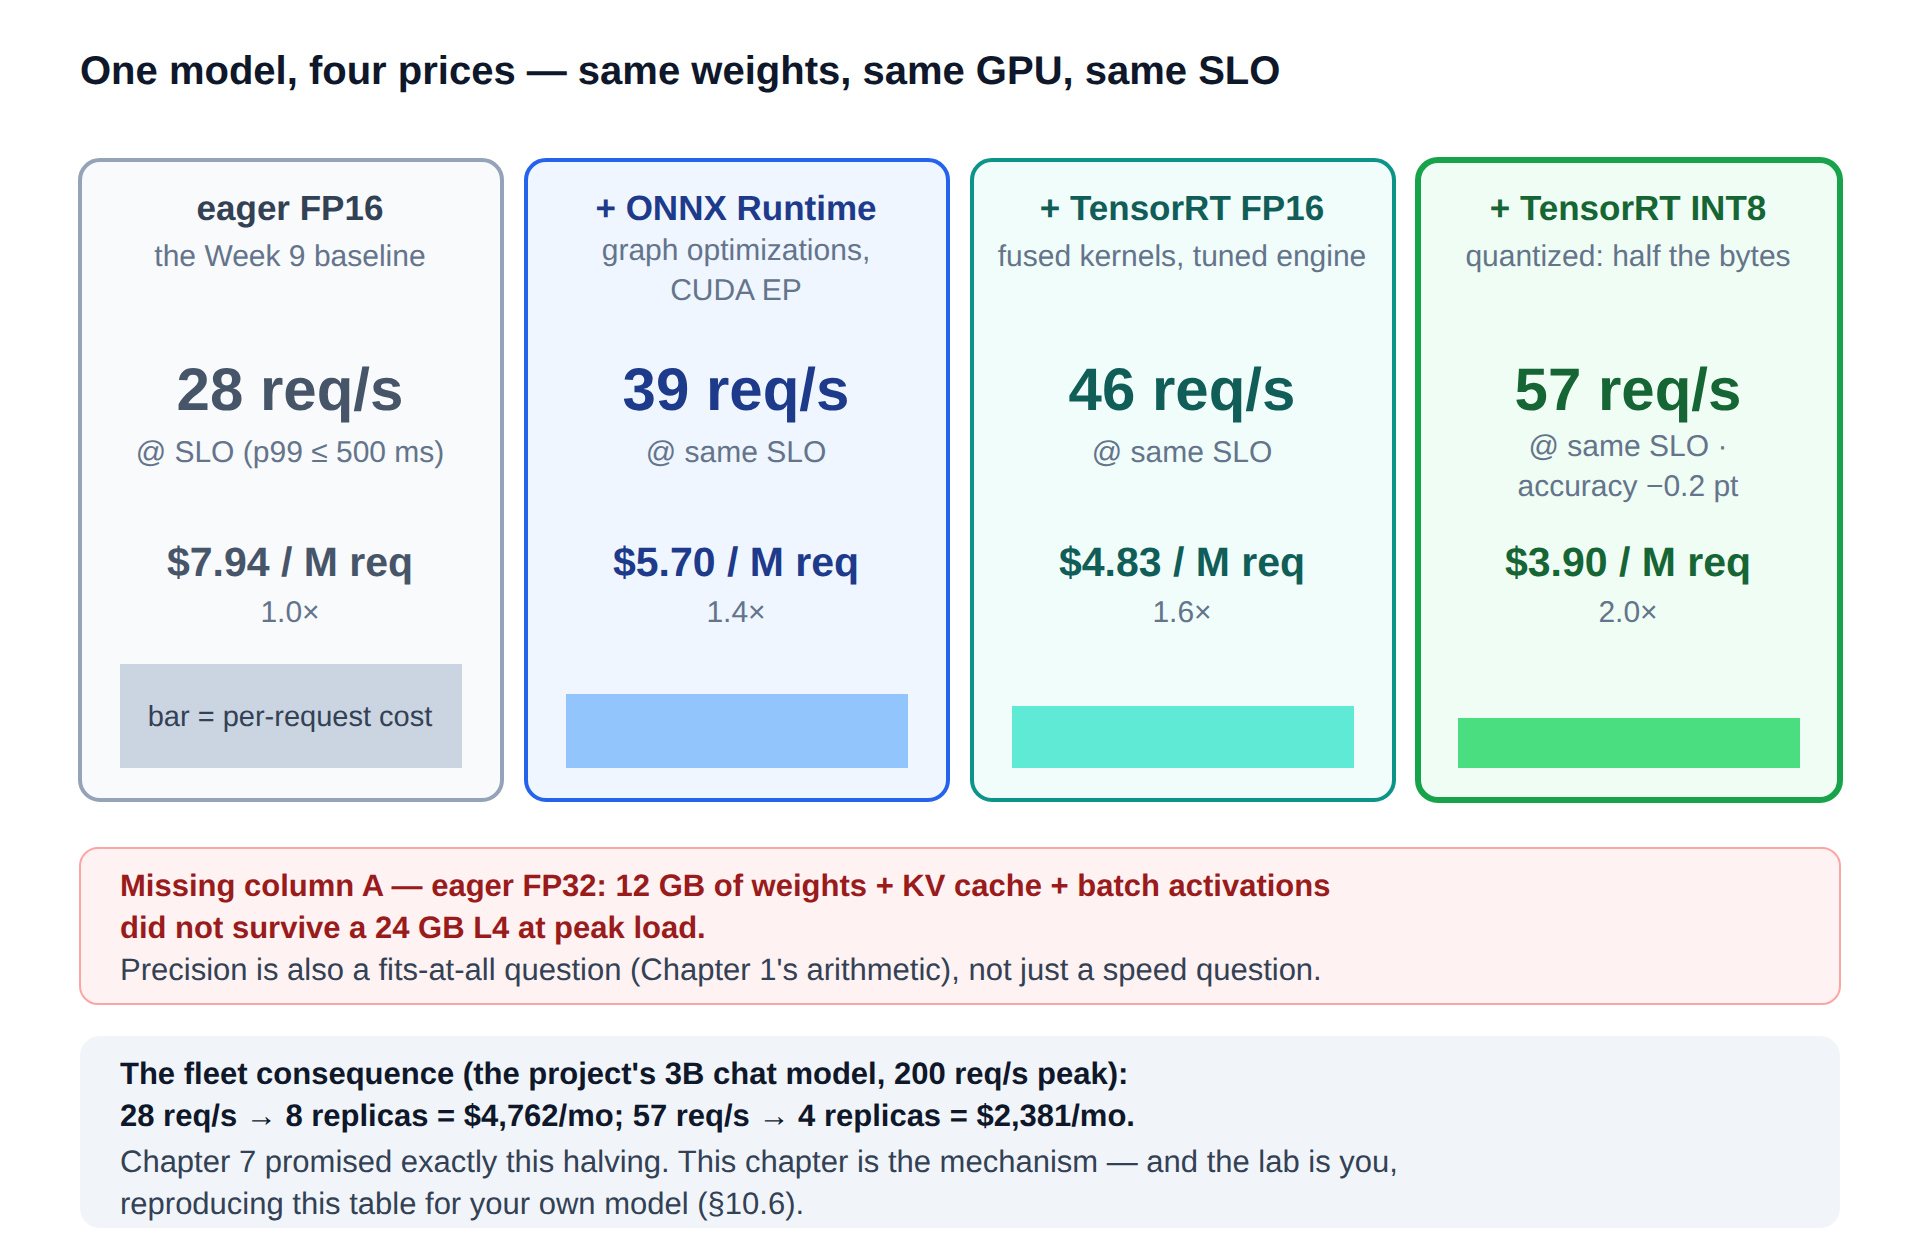
\includegraphics{figures/fig10-1_fourprices.png}}\\[3pt]
  \figcaption{Figure 10-1  Exhibit 10-A, drawn. Same silicon, 2× the goodput per dollar — and the fleet consequence Chapter 7 promised: 8 replicas become 4, \$4,762 becomes \$2,381.}
\end{tbbfigure}

\subsection*{You have trusted lossy compression your whole life}

The idea that you can throw away precision and keep the product sounds reckless until you notice that \textbf{the entire sensory world you consume is already built on it}. When telephone networks digitized voice (the Bell System's T1 carrier, 1962), they did not ship faithful audio: they shipped \textbf{8-bit} samples on a logarithmic ruler (μ-law companding) — 256 levels where the analog signal had infinitely many — because human ears care about ratios, not absolute steps, and 8 well-placed bits sound like a voice. Nobody's mother sounded wrong. Thirty years later \textbf{JPEG (1992)} did it to images — throw away the high-frequency detail eyes barely register, keep a tenth of the bytes, and the vacation photo survives — and \textbf{MP3 (1993)} did it to music with a model of what ears mask. The pattern is always the same: \textit{find what the consumer of the signal actually needs, and stop paying for the rest.}

Quantization is this pattern applied to neural networks, with one beautiful substitution: the "consumer" is not an eye or an ear but \textbf{the model's own decision}. Training genuinely needs fine precision — gradient descent nudges weights by increments of 10⁻⁵ and accumulates them across millions of steps; round those away and learning stalls. But inference asks only that the \textit{outputs} survive: the argmax, the ranking, the generated token. And trained networks turn out to be remarkably tolerant consumers — good minima are flat (nudging every weight by a fraction of a percent barely moves the loss), activations are noisy anyway, and the decision boundaries have margins. Rounding a weight from 0.087231 to 0.0872 is far below the noise the network already shrugs off. \textbf{FP32 for inference is, most of the time, shipping studio-master audio to a phone call} — and §10.3 is about doing the μ-law conversion with the same care Bell Labs did: measure the signal, place the ticks well, and \textit{verify the listener can't tell}.

One more framing before the mechanisms, because it organizes the whole chapter: Chapter 9 left you the two-parameter law \textbf{t(B) = a + b·B} — a fixed cost per pass (launches, scheduling, streaming the weights) and a marginal cost per item (the arithmetic). This chapter is a targeted attack on both constants. \textbf{Compilation shrinks a} (§10.4: fuse the kernels, fold the constants, stop round-tripping activations through memory). \textbf{Quantization shrinks b — and part of a too} (§10.3: half the bytes per weight means the weight-streaming component of every pass halves). And §10.2 explains why \textit{bytes} keep appearing in both sentences: for most inference, the GPU's arithmetic is not the bottleneck at all.

\begin{calloutbox}{tbbpurple}{tbbpurplefill}
{\normalsize\bfseries\color{tbbpurple}Think About It}\par\vspace{3pt}
\begin{tbbitemize}
  \item Exhibit 10-A row A: reconstruct the OOM arithmetic. 3B params × 4 bytes = 12 GB of weights on a 24 GB L4 — walk through what else wants VRAM at peak (batch activations, the chat model's per-sequence KV cache — Ch. 1's memory story, Ch. 9's max\_batch\_size bound) and explain why FP16 (6 GB) made the same server comfortable.
  \item The μ-law analogy has a limit: a phone call degrades gracefully (a slightly muddier voice), while a classifier can flip a decision discretely. Which §10.3 safeguard exists precisely because of that difference — and what is its analog in broadcast engineering, if any?
  \item Row C (ONNX Runtime) gained 1.4× with zero precision change and zero quantization. From what you know after Chapter 9 (a vs. b), where must that win have come from — and which §10.4 mechanism is your prime suspect?
\end{tbbitemize}
\end{calloutbox}

\section{The Memory Wall: Diagnose Before You Optimize}

Every optimization story this chapter tells stands on one unglamorous fact about modern accelerators: \textbf{the math got fast faster than the bytes got close}. A T4 can perform 65 trillion FP16 operations per second, but its memory can deliver only 320 gigabytes in that same second. Divide the two and you get the machine's character: roughly \textbf{200 floating-point operations must arrive per byte fetched} just to keep the compute units from starving. That ratio is the \textit{memory wall} — a name coined back in 1995, when Wulf and McKee noticed that CPU speed was compounding \textasciitilde{}50\% a year while memory access improved \textasciitilde{}7\% and warned, in a famously short paper, that the industry was driving toward a wall at full throttle. GPUs postponed the crash with heroic bandwidth (HBM is the wall's ransom payment), but the ratio kept worsening — and which side of it your workload lives on determines, before any benchmark, which optimizations will pay.

The diagnostic is a single number: \textbf{arithmetic intensity (AI) — FLOPs performed per byte moved}. A workload whose AI exceeds the machine's ratio is \textbf{compute-bound}: the die is genuinely busy, and only cheaper arithmetic helps. A workload below the ratio is \textbf{memory-bound}: the compute units idle while tensors stream in, "faster math" changes nothing, and \textit{fewer bytes} is the only lever that matters. Figure 10-2 draws this as the classic \textbf{roofline}: a slanted bandwidth roof, a flat compute roof, and a ridge where they meet. The uncomfortable news for serving: \textbf{most inference at serving-friendly batch sizes lives left of the ridge} — memory-bound. Batch-1 LLM token generation is the extreme case (every token re-streams every weight for a handful of FLOPs each: AI ≈ 1–10, hopelessly bandwidth-bound — Week 11's entire predicament), while only large-batch CNNs and fat GEMMs reach the compute roof.

\begin{tbbfigure}
  \adjustbox{max width=0.94\linewidth,max totalheight=0.46\textheight}{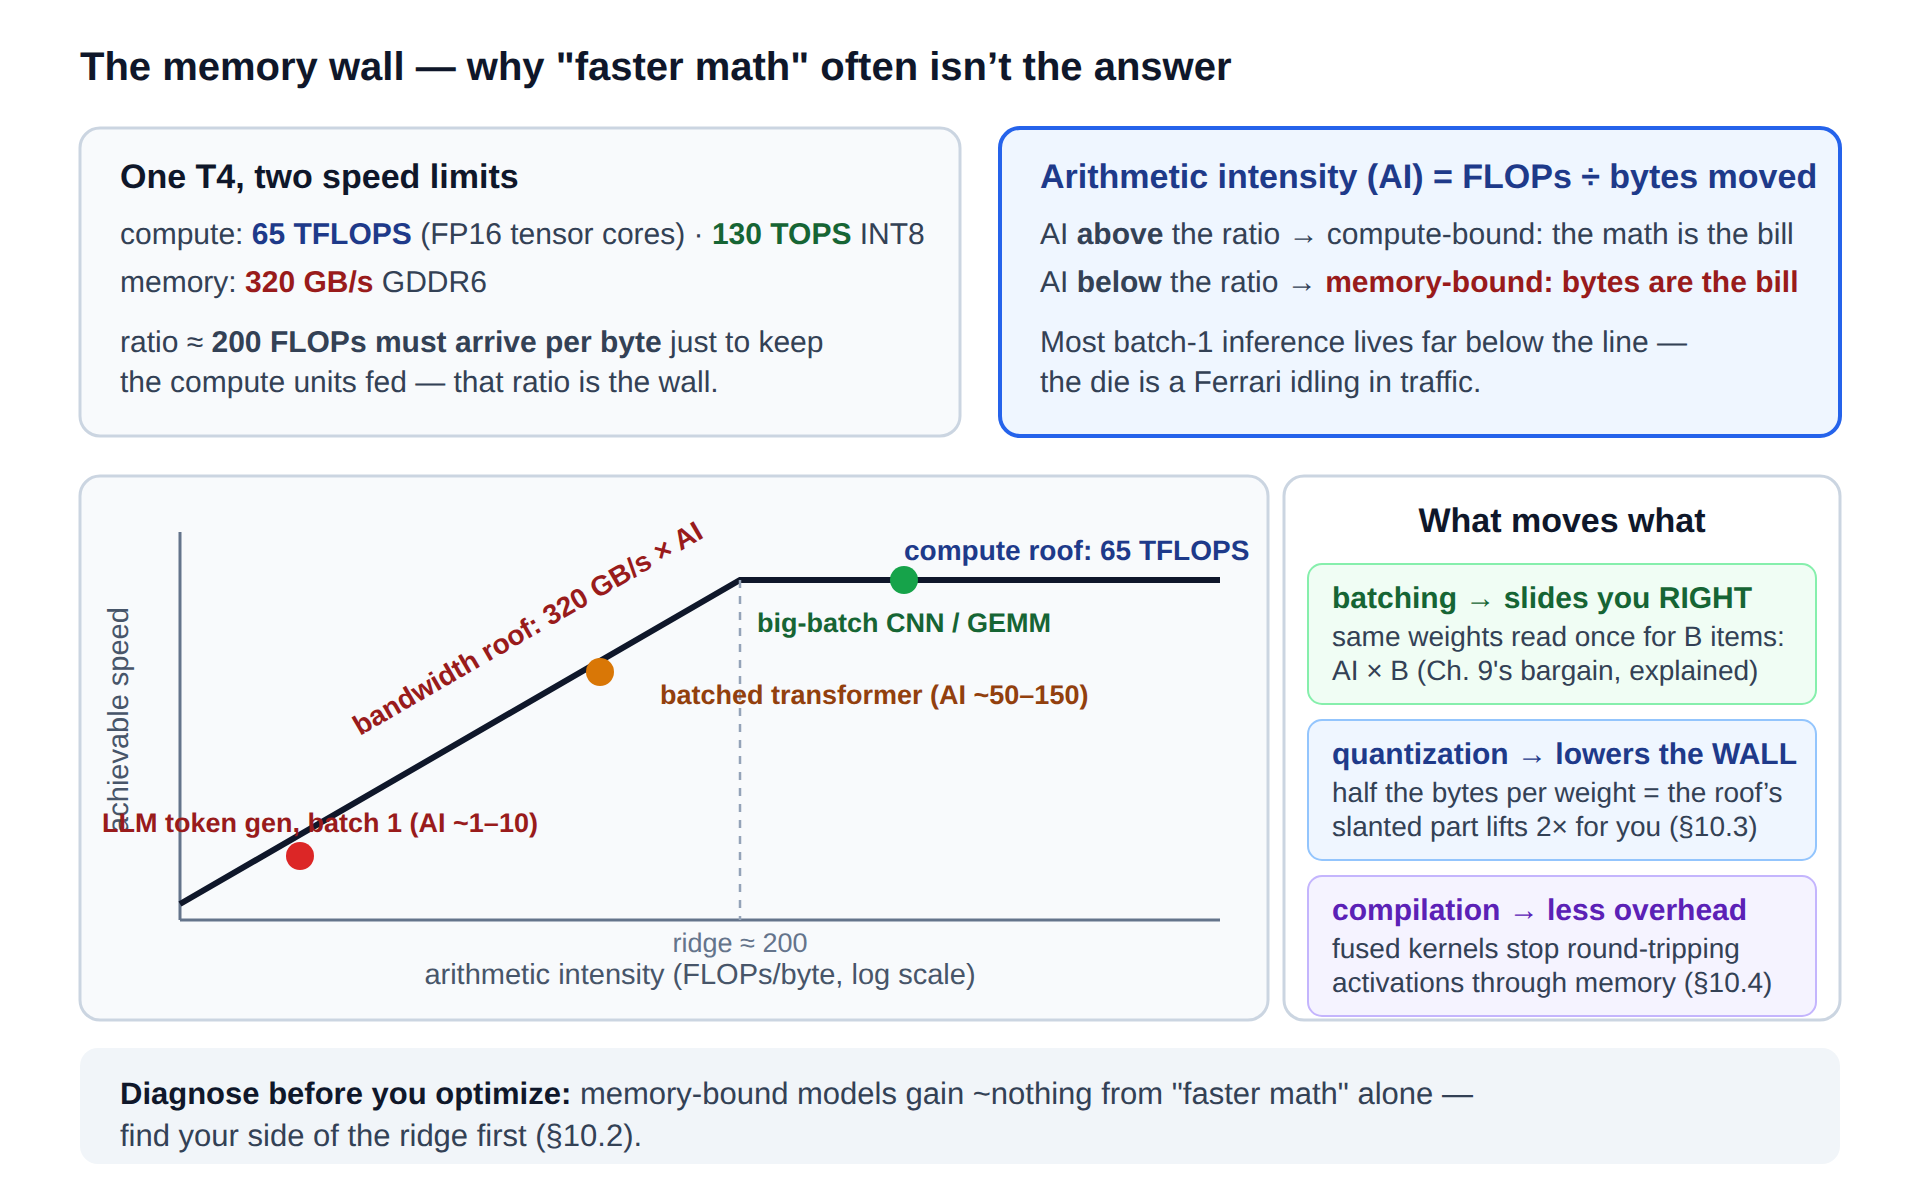
\includegraphics{figures/fig10-2_memorywall.png}}\\[3pt]
  \figcaption{Figure 10-2  The memory wall as a roofline. Batching slides you right (same weights, more work per byte); quantization lifts the slanted roof (fewer bytes per weight); compilation stops wasting trips. Diagnose first — the ridge decides what pays.}
\end{tbbfigure}

\subsection*{The ridge, applied: three workloads you already own}

The definition becomes an instinct once you compute AI for three operations you have been running since Week 2 — so let us do all three, digits showing. \textbf{First, the matrix–vector product that generates a token.} One transformer layer's weight matrix, say 4,096 × 4,096 in FP16, is 33.6 MB; multiplying a single input vector through it performs 2 × 4,096² ≈ 33.6 MFLOP. Divide: \textbf{AI ≈ 1 FLOP per byte} — the weights are read once and used once. Against a ridge of 200, that is not a workload, it is a byte-delivery service with some math attached. Now batch B requests: the same 33.6 MB of weights serves B vectors, FLOPs scale by B, bytes barely move — \textbf{AI ≈ B}. That single line is the entire theory of batching (and of Table 10-3 later): to reach the T4's ridge you would need B ≈ 200, and since the SLO caps this model's batch near 32, generation \textit{lives} memory-bound — which is Week 11's opening problem, met here as arithmetic.

\textbf{Second, ReLU} — max(0, x), one FLOP per element. Each FP16 element must be read (2 bytes) and written (2 bytes): \textbf{AI = 1 ÷ 4 = 0.25}, eight hundred times below the ridge. No hardware ever built runs elementwise ops at anything but memory speed, which is why §10.4's compilers refuse to give ReLU its own kernel at all: fused into the producing op, its bytes simply vanish. \textbf{Third, a real convolution} — 3×3, 64→64 channels on a 56×56 feature map. FLOPs: 2 × 9 × 64 × 64 × 56² ≈ 231 M. Bytes: input 0.40 MB + weights 0.07 MB + output 0.40 MB ≈ 0.88 MB. \textbf{AI ≈ 264} — just \textit{above} the T4's ridge. Convolutions re-use every weight across all 3,136 spatial positions; the data re-use is built into the operation. This is why CNNs are the roofline's good citizens, why the Week 9 classifier's wins will come from math rate and launch overhead rather than weight streaming — and why the same GPU can be starving on one model and sweating on another.

Keep the three numbers — \textbf{≈ B, 0.25, 264} — as your mental furniture: almost every layer you will ever serve is one of these three in costume. You do not need a profiler for the first diagnosis — two lines of arithmetic suffice, and they are the two lines your lab report should open with:

\begin{terminalbox}
\begin{Verbatim}[breaklines=true,breakanywhere=true,fontsize=\small,formatcom=\color{tbbtermfg},codes=\tbbcodeactive]
# is my model memory-bound at this batch size? no profiler needed.
# the project's 3B chat model, on the fleet's L4 (24 GB, 300 GB/s):
# floor set by BYTES: weights must stream once per forward pass:
$ python -c "print(6.0e9 / 300e9 * 1e3, 'ms floor per pass')"
20.0 ms floor per pass      # 3B params x 2B (FP16) / 300 GB/s
# floor set by MATH: ~2 FLOPs/param/item -> batch 1: 6 GFLOP:
$ python -c "print(6.0e9 * 2 / 121e12 * 1e3, 'ms of compute')"
0.1 ms of compute           # vs 20.0 ms of streaming: 200x apart
# verdict: memory-bound by two orders of magnitude at batch 1.
# bytes are the bill. (batch 32 closes the gap ~32x - still bound.)
\end{Verbatim}
\end{terminalbox}
\figcaption{Transcript 10-1  The two-line diagnosis. At batch 1, this model spends 200× longer streaming weights than computing on them — the die is a Ferrari idling in traffic. Every optimization decision downstream follows from this ratio.}

Now re-read Chapter 9's two constants with the wall in view — for \textit{both} of the course's running models, because they sit on opposite sides of it, and the contrast is the whole diagnostic art. For the \textbf{3B chat model}, the fixed cost \textbf{a} is dominated by weight-streaming: 20 ms of unavoidable bytes per pass at FP16 — a floor no compiler can lower, and quantization can halve (INT8 → \textasciitilde{}10 ms). For the \textbf{Week 9 classifier}, the weights are \textasciitilde{}50 MB — 0.16 ms of streaming, a rounding error — so its a = 8.4 ms is almost entirely \textit{launches, scheduling, and per-op overhead}: exactly the waste compilation exists to remove (§10.4), while quantization's gift lands mostly in \textbf{b} (the INT8 math rate, and lighter activation traffic). Batching raised AI by re-using each streamed weight for B items — sliding you rightward along the roofline; that was Chapter 9's bargain. So this chapter's two levers arrive with their assignments already visible: \textbf{quantization attacks bytes} (the slanted roof lifts), \textbf{compilation attacks waste} (launches gone, activations staying in registers instead of round-tripping through VRAM). Diagnosis before optimization is not a platitude; it is why a team that ships "2× faster math" on a memory-bound model measures a 3\% win and a confused afternoon.

\begin{tbbtablewrap}
  \begin{tabular}{@{}>{\raggedright\arraybackslash}m{\dimexpr 0.2021\tbltextwidth-2\tabcolsep\relax} >{\raggedright\arraybackslash}m{\dimexpr 0.1862\tbltextwidth-2\tabcolsep\relax} >{\raggedright\arraybackslash}m{\dimexpr 0.1809\tbltextwidth-2\tabcolsep\relax} >{\raggedright\arraybackslash}m{\dimexpr 0.1915\tbltextwidth-2\tabcolsep\relax} >{\raggedright\arraybackslash}m{\dimexpr 0.2394\tbltextwidth-2\tabcolsep\relax}@{}}
  \arrayrulecolor{tbbnavy}\specialrule{1pt}{0pt}{0pt}
  \rowcolor{tbbtablehead}{\centering \bfseries\color{tbbnavy}GPU (VRAM)} & {\centering \bfseries\color{tbbnavy}FP16 tensor math} & {\centering \bfseries\color{tbbnavy}Memory bandwidth} & {\centering \bfseries\color{tbbnavy}Ridge (FLOPs/byte)} & {\centering \bfseries\color{tbbnavy}Role in this course} \\
  \arrayrulecolor{tbbnavy}\specialrule{0.7pt}{0pt}{2pt}
  {\textbf{T4 (16 GB)}} & {65 TFLOPS} & {320 GB/s} & {≈ 200} & {The lab card — sweeps, INT8 at 2× rate (130 TOPS)} \\
  \arrayrulecolor{tbbtableborder}\hline
  {\textbf{L4 (24 GB)}} & {121 TFLOPS} & {300 GB/s} & {≈ 400} & {The fleet card — Exhibit 10-A, the \$0.80/hr bill} \\
  \arrayrulecolor{tbbtableborder}\hline
  {\textbf{A100 (80 GB)}} & {312 TFLOPS} & {2,039 GB/s} & {≈ 153} & {The think-question card — bandwidth is the premium} \\
  \arrayrulecolor{tbbtableborder}\hline
  {\textbf{H100 (80 GB)}} & {\textasciitilde{}990 TFLOPS} & {3,350 GB/s} & {≈ 295} & {Frontier reference — Week 11's FP8 lives here} \\
  \arrayrulecolor{tbbnavy}\specialrule{1pt}{2pt}{0pt}
  \end{tabular}\par
  \figcaption{Table 10-1  The course's machines, read as ratios (approximate published specs; the ridge = TFLOPS ÷ bandwidth is the number to remember)}
\end{tbbtablewrap}

Read the table as ratios and three lessons fall out. First, \textbf{the ridge is not a constant of nature} — it is a design choice, and it varies 2.5× across cards you can rent this afternoon. The L4 is the starkest: it doubles the T4's math while \textit{lowering} its bandwidth, parking the ridge near 400 — a card built to be fed INT8 at healthy batch sizes, and predictably miserable at batch-1 FP16 generation (Exhibit 10-A's row B, explained by silicon). Second, \textbf{the A100's premium is mostly bandwidth}: \textasciitilde{}5× the T4's math but \textasciitilde{}6.4× its bytes — re-run Transcript 10-1 on it and the streaming floor falls from 20 ms to 2.9 ms while the compute floor barely matters; for memory-bound inference, expensive GPUs are expensive \textit{memory} with math attached. Third, the generation-over-generation drift is \textit{upward} — the wall keeps getting taller — which means \textbf{quantization becomes more valuable with every hardware generation, not less}: bytes are the appreciating currency. (This is also why Hopper-class cards added FP8 as a first-class format — the hardware itself is begging you to send fewer bytes; §10.3 obliges.)

\subsection*{The other wall: PCIe, and the trip the bytes take first}

The roofline's 300 GB/s is the \textit{inner} wall — VRAM to compute units. There is an outer one, and Chapter 6 left you standing at it: the weights arrived from the object store into \textbf{host page cache} (mmapped safetensors, the kernel paging tensors in on first touch), and we promised this chapter would finish the trip. The last leg is a \textbf{host-to-device (H2D) copy across PCIe} — and PCIe is the slowest road in the machine: a gen3 ×16 slot moves \textasciitilde{}16 GB/s theoretical, half to a third of what it delivers in practice depending on how you ask. The asking matters because of Chapter 3's memory machinery: the GPU's DMA engine can only pull from \textbf{pinned (page-locked) memory} — pages the kernel promises never to swap or move. Copy from ordinary pageable memory and CUDA silently stages everything through an internal pinned bounce buffer — one extra memcpy, roughly half the throughput. Pin the buffer yourself and the DMA engine reads it directly:

\begin{terminalbox}
\begin{Verbatim}[breaklines=true,breakanywhere=true,fontsize=\small,formatcom=\color{tbbtermfg},codes=\tbbcodeactive]
# how fast can bytes actually get INTO the GPU? (lab T4, PCIe gen3 x16)
$ python h2d_bench.py --mb 256
  pageable host -> device    6.3 GB/s   # malloc'd memory: CUDA stages
                                        # it through a pinned bounce buffer
  pinned   host -> device   12.6 GB/s   # page-locked: DMA reads directly
  VRAM     device internal 298.1 GB/s   # the inner wall, for scale: ~25x
# lesson 1: PCIe is ~25x slower than VRAM. weights cross ONCE, at startup,
#           and live in VRAM. nothing model-sized crosses per request.
# lesson 2: pin what does cross (DataLoader/serving: pin_memory=True),
#           and overlap copy with compute (CUDA streams - free otherwise).
\end{Verbatim}
\end{terminalbox}
\figcaption{Transcript 10-2  The outer wall, measured. Pageable copies pay a hidden staging memcpy; pinned memory doubles H2D throughput; and both are dwarfed by VRAM bandwidth — which is why residency, not transfer speed, is the design rule.}

This is Chapter 2's lab observation, finally explained from below: your batch-1 GPU benchmark underwhelmed because tiny work pays the PCIe hop and the launch overhead without amortizing either. And it completes the model's journey as a supply chain with three speeds — \textbf{object store → host page cache (GB/s, once per pod, §6.4) → VRAM (12 GB/s pinned, once per process) → compute units (300 GB/s, every single pass)} — each stage roughly an order of magnitude faster than the one before, each crossed proportionally less often. The design rules write themselves: weights cross PCIe exactly once (startup — the cold-start path Chapter 5 budgeted); per-request tensors are small (an image \textasciitilde{}150 KB, a prompt a few KB — at 12 GB/s, tens of microseconds) but must be pinned and asynchronous or they serialize; and results cross back. Serving frameworks (Chapter 9's organ ⑤) do the pinning and stream-overlap for you — the reason to know the mechanism is Chapter 9's §9.4 lesson: when the framework's defaults are wrong, the two-line diagnosis now has a third line, and \code{nvidia-smi dmon}'s PCIe columns are where you look.

\begin{calloutbox}{tbbpurple}{tbbpurplefill}
{\normalsize\bfseries\color{tbbpurple}Think About It}\par\vspace{3pt}
\begin{tbbitemize}
  \item Run Transcript 10-1's two lines for an A100-80GB (312 TFLOPS FP16, \textasciitilde{}2,000 GB/s) serving the same 3B model. Which floor moved more, and what does that say about where expensive GPUs earn their premium for inference?
  \item A teammate proposes upgrading the fleet to a GPU with "4× the TFLOPS" (similar bandwidth) to fix latency on your batch-4 LLM endpoint. Use the wall to predict the outcome in one sentence — and name the two purchases that WOULD move the number.
  \item Why does batching "slide you right" rather than "lift the roof"? State, in bytes and FLOPs, what changes when B goes from 1 to 16 — and what does NOT change. (This is Ch. 9's a + b·B, re-expressed.)
  \item A video-inference service sends 90 MB of decoded frames per request. Using Transcript 10-2's numbers, compute the H2D time pageable vs. pinned, compare both to the model's 11 ms forward pass — and name the two §10.2 remedies before anyone touches the model.
\end{tbbitemize}
\end{calloutbox}

\section{Quantization: Coarser Rulers, Gated Honestly}

Quantization is mechanically humble: \textbf{re-express tensors on a ruler with fewer ticks}. An FP32 weight is one of \textasciitilde{}4 billion representable values spread across a huge dynamic range; the weights of any given layer, meanwhile, huddle in a tiny interval (±0.4 is typical — Figure 10-3's bell). INT8 quantization lays a 256-tick ruler over exactly that interval — \textbf{q = round(w / scale) + zero\_point} — storing one byte per weight plus a handful of scale parameters. Dequantization multiplies back at compute time, or — better, and the reason this chapter's numbers double instead of merely shrinking storage — the hardware \textbf{computes directly in INT8} (a T4's tensor cores run INT8 at twice the FP16 rate: 130 TOPS), so both floors of Transcript 10-1 drop at once: half the bytes to stream, double the math throughput.

\begin{tbbfigure}
  \adjustbox{max width=0.94\linewidth,max totalheight=0.46\textheight}{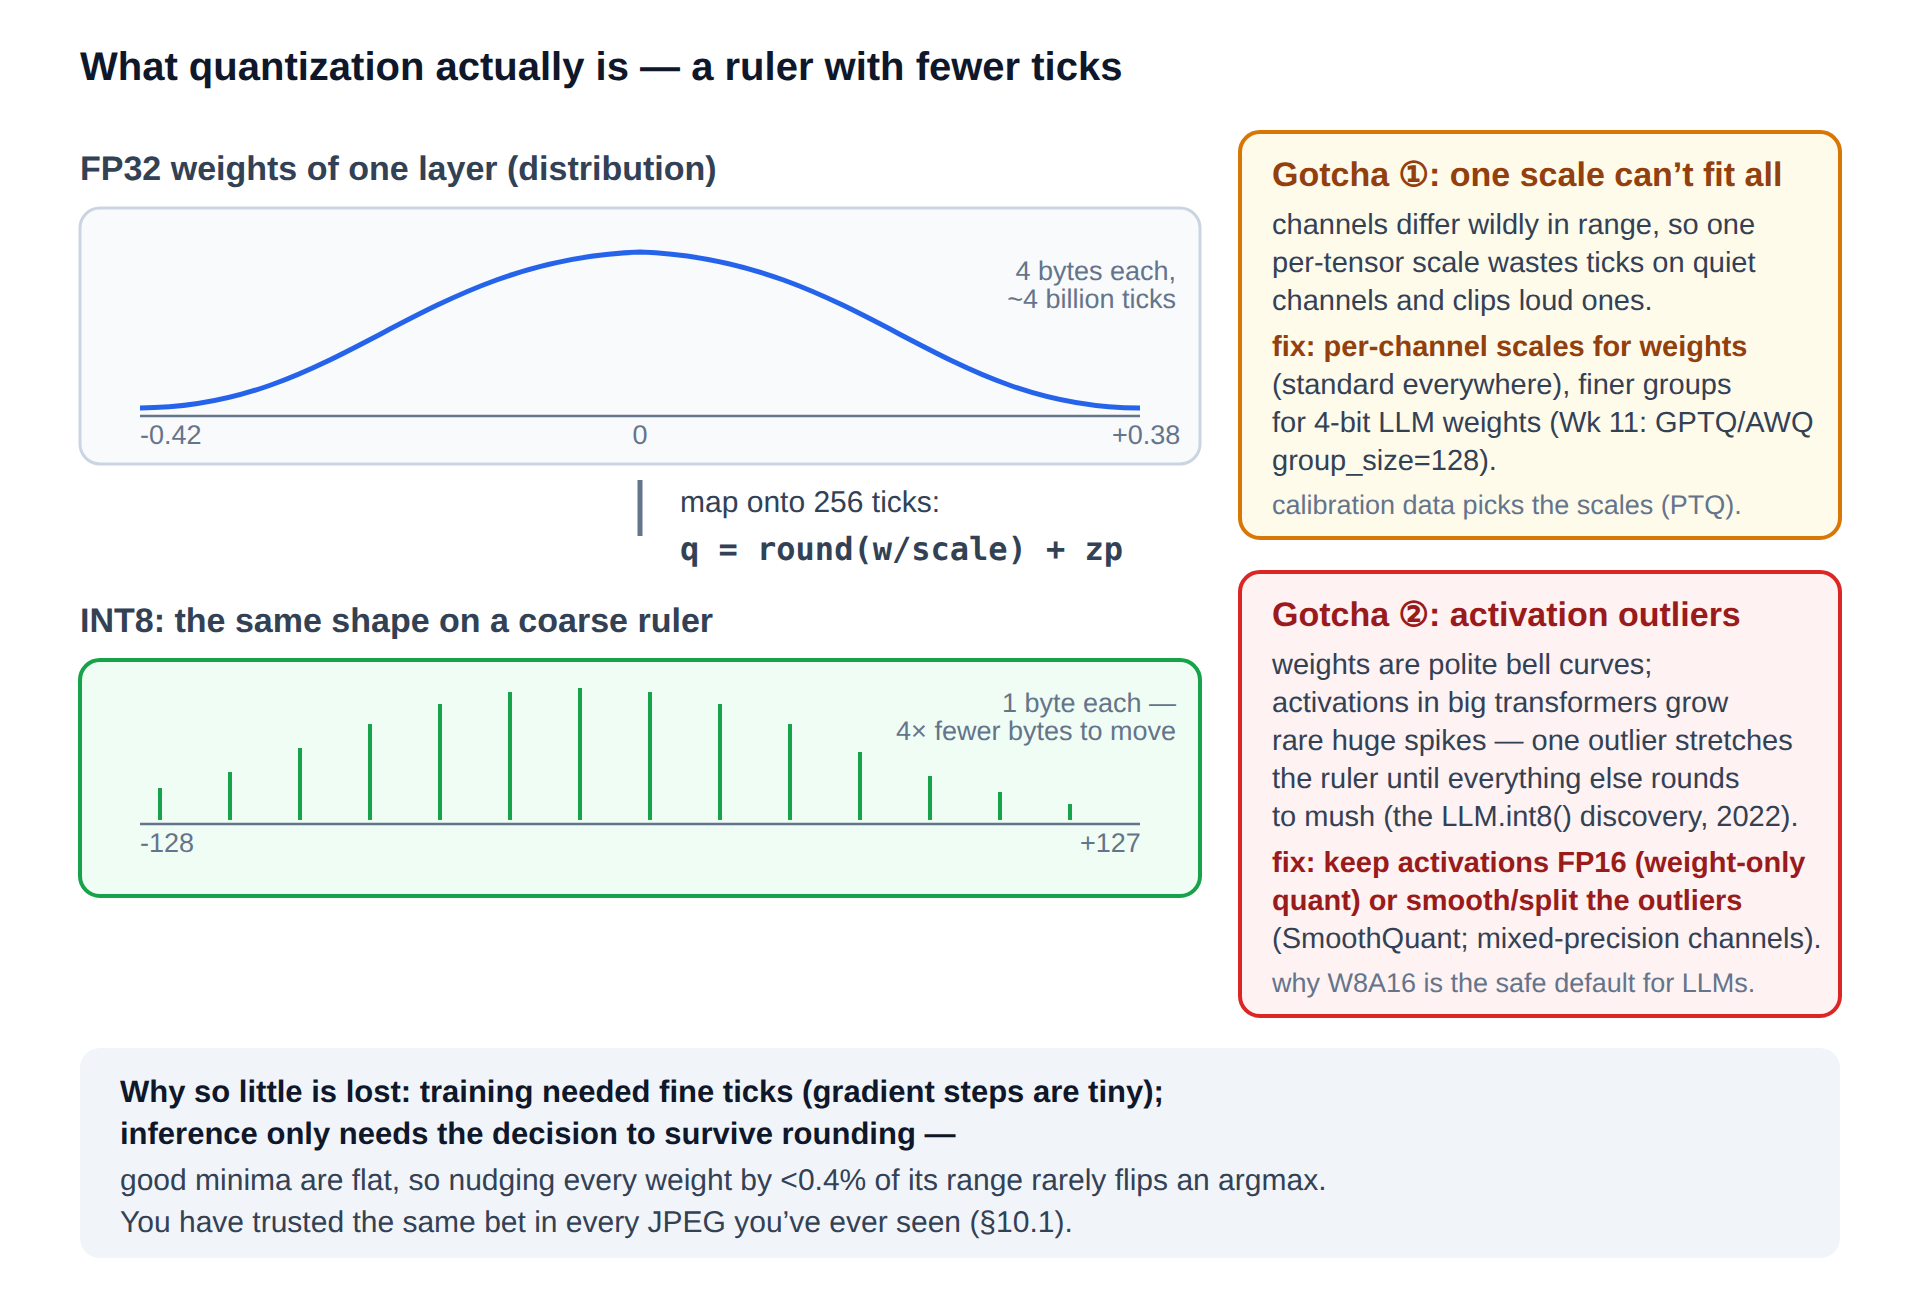
\includegraphics{figures/fig10-3_quantmap.png}}\\[3pt]
  \figcaption{Figure 10-3  Quantization is a coarser ruler over the range the tensor actually uses. The craft is placing the ticks (scales, per-channel), and the two gotchas: ranges differ per channel, and transformer activations hide outliers.}
\end{tbbfigure}

\subsection*{The rulers themselves: why floats forgive and integers don't}

Before placing ticks, look at what the ticks are made of, because the whole difficulty of this section comes from one structural difference. A \textbf{floating-point number carries its own ruler}: the exponent bits scale each value individually (a number near 0.001 and a number near 1,000 each get their mantissa's full resolution), which is why you have spent five weeks of labs never once thinking about ranges. An \textbf{integer has no exponent} — it is a bare position on one fixed ruler, so \textit{somebody else} must choose that ruler's span, once, for the whole tensor. That somebody is calibration, and every gotcha below (channels that differ, outliers that stretch) is a consequence of many values being forced to share one scale. Floats forgive; integers delegate the forgiveness to you.

The float family is worth thirty seconds because its members now appear on every GPU spec sheet. \textbf{FP32} (1 sign · 8 exponent · 23 mantissa) is the reference ruler. \textbf{FP16} (1·5·10) halves the bytes but shrinks the \textit{range} — max 65,504 — which is why training in FP16 needs loss-scaling tricks to keep small gradients from flushing to zero. \textbf{BF16} (1·8·7) makes the opposite trade: it keeps FP32's full exponent range and pays with a coarse mantissa (\textasciitilde{}3 decimal digits) — gradients never overflow, so it became training's darling; for \textit{serving} it is rarely a win over FP16 (same 2 bytes, same speed on most GPUs). \textbf{FP8} (Hopper/Ada hardware: H100, and the fleet's L4 has the circuits) comes in two cuts — E4M3 (±448, for weights and activations) and E5M2 (±57,344, for gradients) — and is best understood as \textit{integer-cost storage with a little self-scaling left in}: still calibrated in practice, but far more tolerant of imperfect scales than INT8. And \textbf{INT8/INT4} are the bare rulers of this chapter: cheapest, fastest, and entirely dependent on the tick-placement craft below.

One implementation footnote that saves a recurring confusion: inside an INT8 layer, the INT8 × INT8 products are \textbf{accumulated in INT32} — thousands of terms sum without overflow — and the result is \textit{requantized} to the output's scale on the way out. Accuracy problems in quantized models are therefore essentially never "the accumulator overflowed"; they are always "the ticks were placed badly for this tensor." Diagnose accordingly: the fix lives in scales and calibration, not in arithmetic width.

\subsection*{Placing the ticks: scales, granularity, calibration}

Watch the mechanism once with real numbers, because it fits in four lines and demystifies every acronym that follows. Take a layer whose weights span [−0.42, +0.38]. Symmetric INT8 uses ticks −127…+127, so \textbf{scale = max|w| ÷ 127 = 0.42 ÷ 127 ≈ 0.00331} (zero\_point = 0). The weight 0.087231 becomes q = round(0.087231 ÷ 0.00331) = \textbf{26}; stored in one byte; dequantized at compute time to 26 × 0.00331 = 0.08606. The rounding error — about 0.0012, a third of one tick — is the entire "loss" everyone debates, and it lands \textit{below} the noise floor the network already tolerates (§10.1's flat-minima argument, now with digits). The whole 25 MB FP32 layer becomes \textasciitilde{}6.3 MB plus a few float scales. That is all quantization \textit{is}; everything else in this section — granularity, calibration, outliers, the gate — is about the cases where this four-line story goes wrong.

The example used a \textit{symmetric} ruler (zero\_point = 0) because weights straddle zero. Activations often do not: after a ReLU, a layer's outputs might span \textbf{[0, 6.2]} — and a symmetric ruler would spend half its 256 ticks on negative values that never occur, doubling the step size for no reason (6.2 ÷ 127 = 0.049). The \textbf{zero\_point} exists for exactly this: an \textit{asymmetric} ruler sets scale = 6.2 ÷ 255 = 0.024 and zero\_point = −128, mapping real 0.0 to code −128 — all 256 ticks now cover the range that actually happens, at half the step. This is the entire job of that mysterious second parameter in q = round(w/scale) + zero\_point: it slides the ruler so none of it is wasted.

All quantization craft is tick placement. \textbf{One scale per tensor} is the bluntest choice, and the arithmetic shows how blunt: suppose channel 7's weights span ±2.0 while channel 300's span ±0.05. The shared scale must accommodate channel 7, so scale = 2.0 ÷ 127 ≈ 0.0157 — and now channel 300's \textit{entire life} happens inside about three ticks. Its typical weight 0.02 quantizes to q = round(0.02 ÷ 0.0157) = 1, dequantizes to 0.0157 — a \textbf{21\% error}, on every weight, systematically. Give channel 300 its own ruler (scale = 0.05 ÷ 127 ≈ 0.00039) and the same weight becomes q = 51 → 0.0201: \textbf{0.4\% error}, fifty times better, for the cost of one extra float per channel. Hence \textbf{per-channel scales} (one ruler per output channel) are the universal standard for weights, and 4-bit LLM quantization goes finer still with \textbf{per-group scales} (one per 128 weights — Week 11's GPTQ/AWQ vocabulary, met here in passing). Where do the ranges come from? For weights, from the file — they are known constants. For \textit{activations}, someone must observe them: \textbf{calibration} runs a few hundred representative inputs through the model, records each layer's activation ranges, and picks scales accordingly. This is \textbf{post-training quantization (PTQ)} — no retraining, minutes in CI — and its quality is exactly the quality of the calibration set: calibrate an image model on daytime photos only, and nighttime inputs will clip. (The alternative, \textbf{quantization-aware training (QAT)}, simulates rounding during fine-tuning so the network learns around it; it recovers accuracy PTQ loses, at training-pipeline prices. This course's road is PTQ; know when to reach past it — Figure 10-4.)

How does calibration turn a pile of observed activations into one scale? Three recipes, in ascending sophistication — and the difference is not academic. \textbf{Min–max} takes the literal extremes: honest, and fragile — if 999 activations live under 6.0 but one freak value hits 41.0, the scale becomes 41 ÷ 127 ≈ 0.32, and the entire real population now squeezes into about \textbf{nineteen ticks} (6 ÷ 0.32) of the 127 available. One weird input just cost you three bits of resolution, permanently. \textbf{Percentile} (say, the 99.99th) clips the freaks: scale = 6.3 ÷ 127 ≈ 0.05, the population gets its full ruler back, and the rare 41.0 saturates at the top tick — a bounded error on a rare value, traded for resolution on everything else. Almost always the right trade. \textbf{Entropy/KL calibration} (TensorRT's default) automates the trade: it sweeps candidate clip thresholds and keeps the one that minimizes the information lost between the FP32 distribution and its INT8 shadow. Whichever recipe you choose, remember the hierarchy: the \textit{method} tunes the ruler within the calibration set's world — but the \textit{set} defines that world, which is why the daytime/nighttime failure above outranks any recipe choice.

The second gotcha earns its own paragraph because it shaped the modern LLM stack. Weights are polite bell curves; \textbf{activations in large transformers are not} — a few channels produce rare, huge spikes (\textasciitilde{}100× the typical magnitude), a phenomenon made famous by the LLM.int8() work in 2022. One outlier stretches the ruler until every normal value rounds to mush; quantize activations naively and a 13B model's perplexity detonates. The practical responses, in the order you will meet them: \textbf{weight-only quantization} (store weights in INT8/INT4, compute in FP16 — since §10.2 showed weights dominate the bytes, most of the win survives; this is the LLM default), \textbf{smoothing} (SmoothQuant-style rescaling that shifts range pressure from activations into weights before quantizing both), and \textbf{mixed precision} (keep the outlier channels in FP16). For this week's CNN-class lab model, activations are tame and full W8A8 INT8 works; file the outlier story where Week 11 will need it.

\begin{tbbfigure}
  \adjustbox{max width=0.94\linewidth,max totalheight=0.46\textheight}{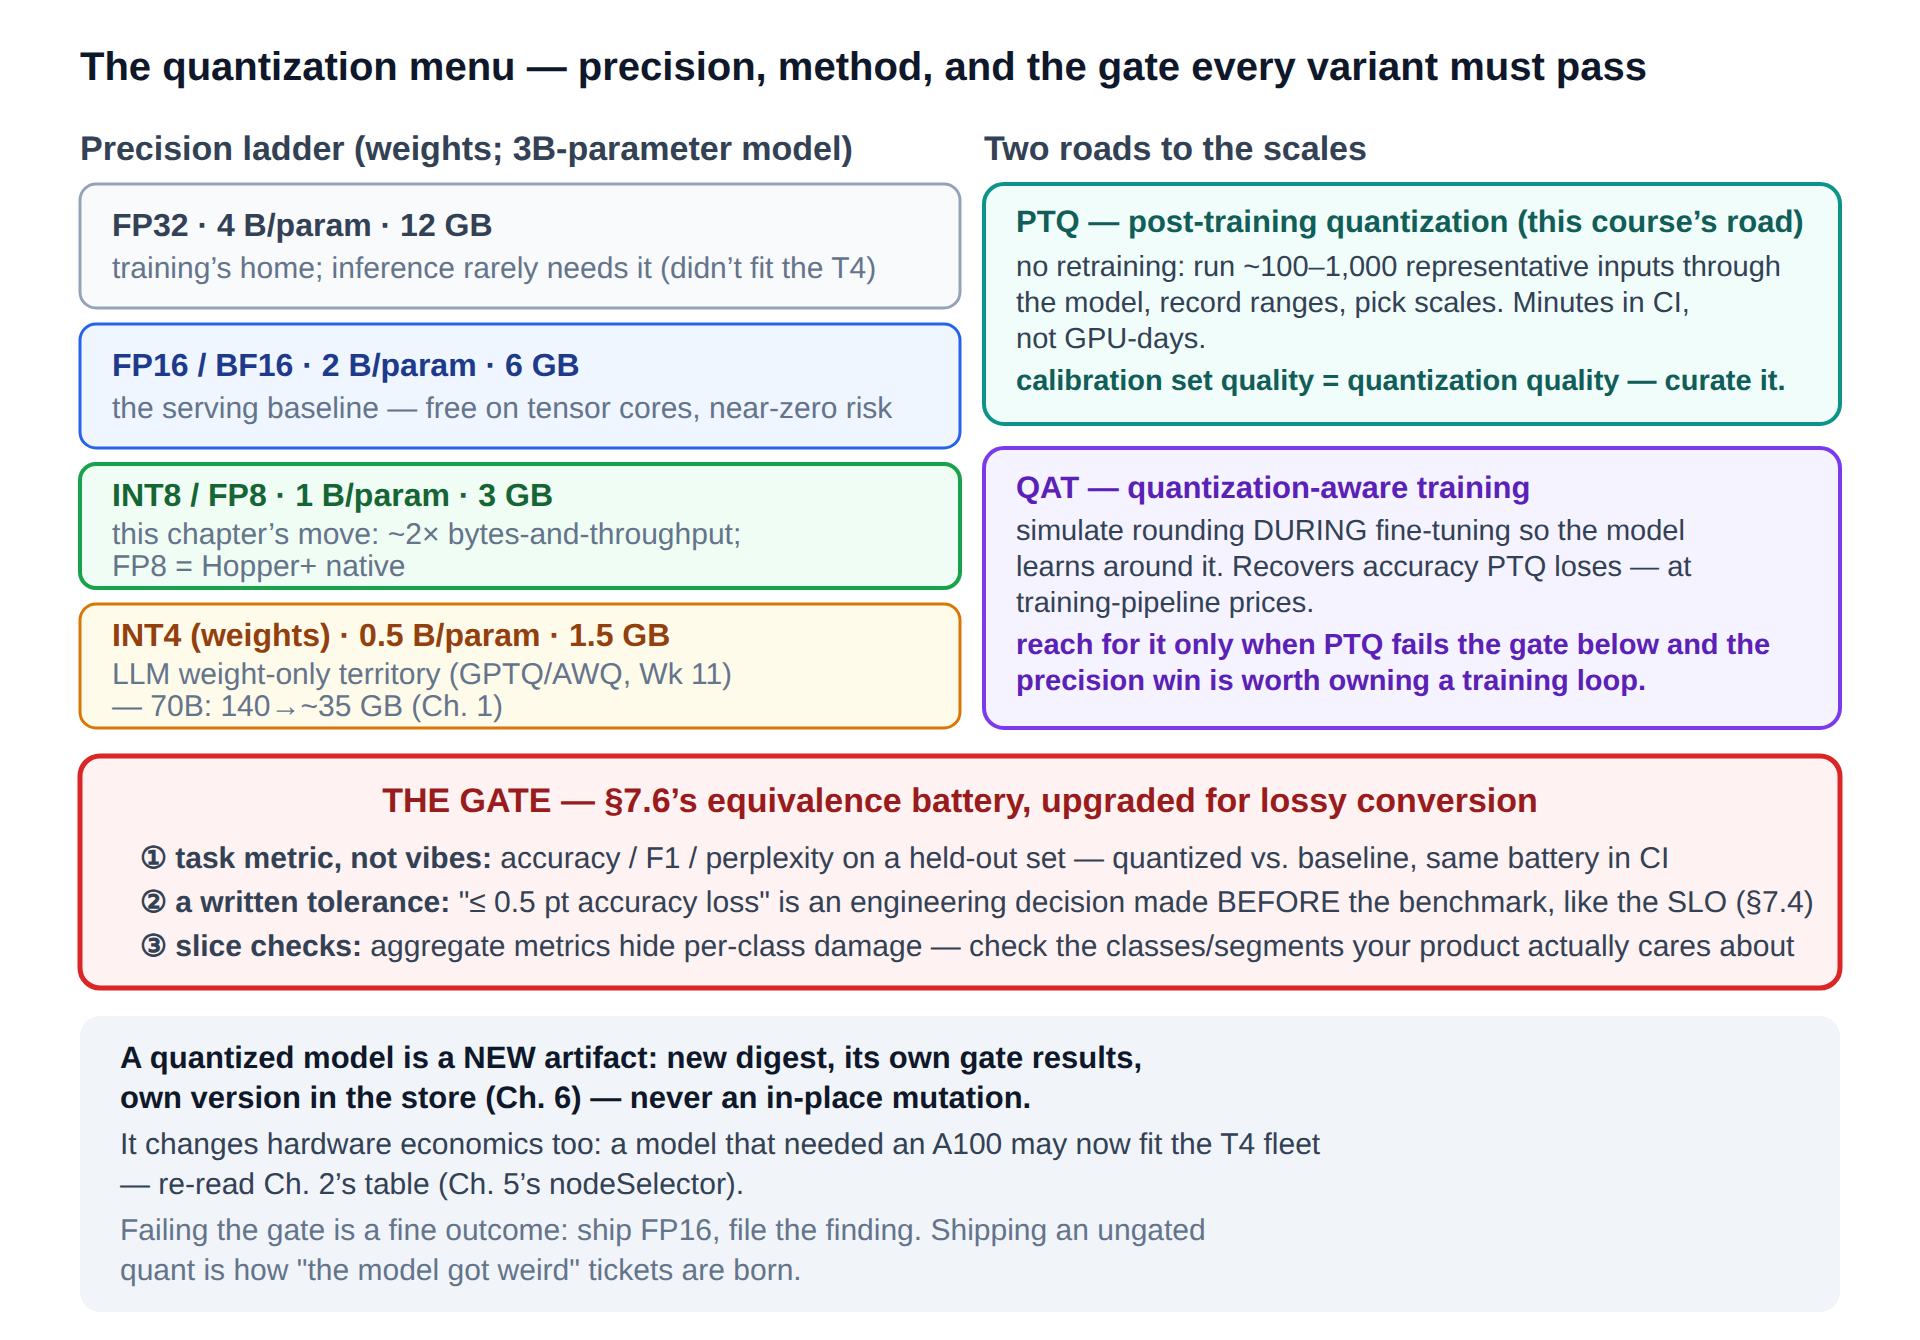
\includegraphics{figures/fig10-4_quantmenu.png}}\\[3pt]
  \figcaption{Figure 10-4  The menu and the gate. Precision ladder (with Chapter 1's 70B: 140 GB → \textasciitilde{}35 GB at INT4), PTQ vs. QAT — and the gate every lossy artifact must pass before it earns a version.}
\end{tbbfigure}

\subsection*{The gate: how a lossy artifact earns the right to ship}

Row E of Exhibit 10-A is only engineering because of what happened before anyone saw its throughput: the \textbf{gate}. A quantized model is a \textit{changed} model — §7.6's equivalence battery, built for lossless-in-spirit conversions, upgrades for lossy ones. Three parts. \textbf{A task metric, not vibes}: accuracy, F1, or perplexity on a held-out set, quantized versus baseline, run by CI, not by whoever is excited. \textbf{A written tolerance}: "≤ 0.5 points top-1 loss" is an engineering decision made \textit{before} the benchmark — the accuracy analog of the SLO, and like the SLO it converts arguments into arithmetic. \textbf{Slice checks}: aggregates hide concentrated damage — a 0.2-point global dip can be a 4-point crater on the one class your product exists for, so the gate checks the slices someone cares about. Transcript 10-3 shows a passing run:

\begin{terminalbox}
\begin{Verbatim}[breaklines=true,breakanywhere=true,fontsize=\small,formatcom=\color{tbbtermfg},codes=\tbbcodeactive]
$ python gate.py --baseline clf_fp16 --candidate clf_int8 --tol 0.5
held-out set: 10,000 images (never seen by calibration)
  baseline   top-1  76.14%
  candidate  top-1  75.92%     delta -0.22 pt   (tol 0.5)  PASS
  worst slice: "streetcar" -1.8 pt  (slice fail-line 3.0)  flag
  logit drift |p99|: 0.041
verdict: PROMOTE -> s3://models/clf/v8-int8/  (new digest)
# fail path exists and is honorable: ship FP16, file the finding.
# an ungated quant is how "the model got weird" tickets are born.
\end{Verbatim}
\end{terminalbox}
\figcaption{Transcript 10-3  The gate, passing. The tolerance was written before the run; the slice check looked where aggregates hide damage; and the output is a NEW artifact with its own digest — never an in-place mutation of the old one.}

Two operational corollaries close the section. \textbf{A quantized model is a new artifact}: new digest, its own gate report stored beside it, its own version in the model store (Chapter 6) — the store's versions-side-by-side design (Chapter 9, organ ④) exists for exactly this rollback story. And \textbf{quantization re-prices hardware}: a model that demanded an A100's VRAM may now fit the T4 fleet, Chapter 1's 70B poster child drops from 140 GB to \textasciitilde{}35 GB at INT4 (four cheap GPUs' worth, or one big one) — so re-read Chapter 2's fleet table after every precision change; Chapter 5's \code{nodeSelector} question ("which GPU label do we aim at?") has a new right answer, and the binding dimension may have moved.

\begin{calloutbox}{tbbpurple}{tbbpurplefill}
{\normalsize\bfseries\color{tbbpurple}Think About It}\par\vspace{3pt}
\begin{tbbitemize}
  \item Your calibration set is 500 images sampled from last month's traffic. The product launches in a new country next week. Explain the failure mode PTQ has just been set up for, the §10.3 knob it corresponds to (tick placement), and the cheap mitigation.
  \item Write the gate sentence for YOUR project model: metric, held-out set, tolerance, and the one slice you would insist on checking. Then defend the tolerance number to a skeptical teammate — where did it come from?
  \item Weight-only INT4 keeps activations in FP16, so the arithmetic is unchanged — yet batch-1 LLM latency improves nearly 4×. Reconcile this with §10.2 in two sentences. (Which floor moved?)
  \item A vendor claims "INT8 with zero accuracy loss, guaranteed, no calibration needed." Using this section, list the three questions that expose what the claim must actually mean.
  \item BF16 keeps FP32's exponent and throws away 16 bits of mantissa; FP16 keeps more mantissa and throws away range. From the "rulers themselves" subsection, explain why BF16 won training, why neither wins \textit{serving} over the other — and what FP8-E4M3 offers that INT8 cannot.
\end{tbbitemize}
\end{calloutbox}

\section{Graph Compilation: Fewer Trips, Fewer Launches}

Quantization shrank the bytes; compilation attacks the \textit{waste} — and to see the waste, watch eager execution do its honest, naive thing. Eager PyTorch runs your model as Python encounters it: each operation launches its own GPU kernel, reads its inputs from VRAM, writes its outputs back. For a conv → batch-norm → ReLU → add chain, that is four kernel launches (each a fixed cost — a slice of Chapter 9's \textbf{a}) and, worse for a memory-bound world, \textbf{three round-trips of the intermediate activations through VRAM} — the very bytes §10.2 taught you to treat as the bill, spent on values that live for microseconds. Eager's flexibility (any Python, any control flow) is why you prototype in it; this section is about what happens when you stop paying for flexibility you no longer use.

\begin{tbbfigure}
  \adjustbox{max width=0.94\linewidth,max totalheight=0.46\textheight}{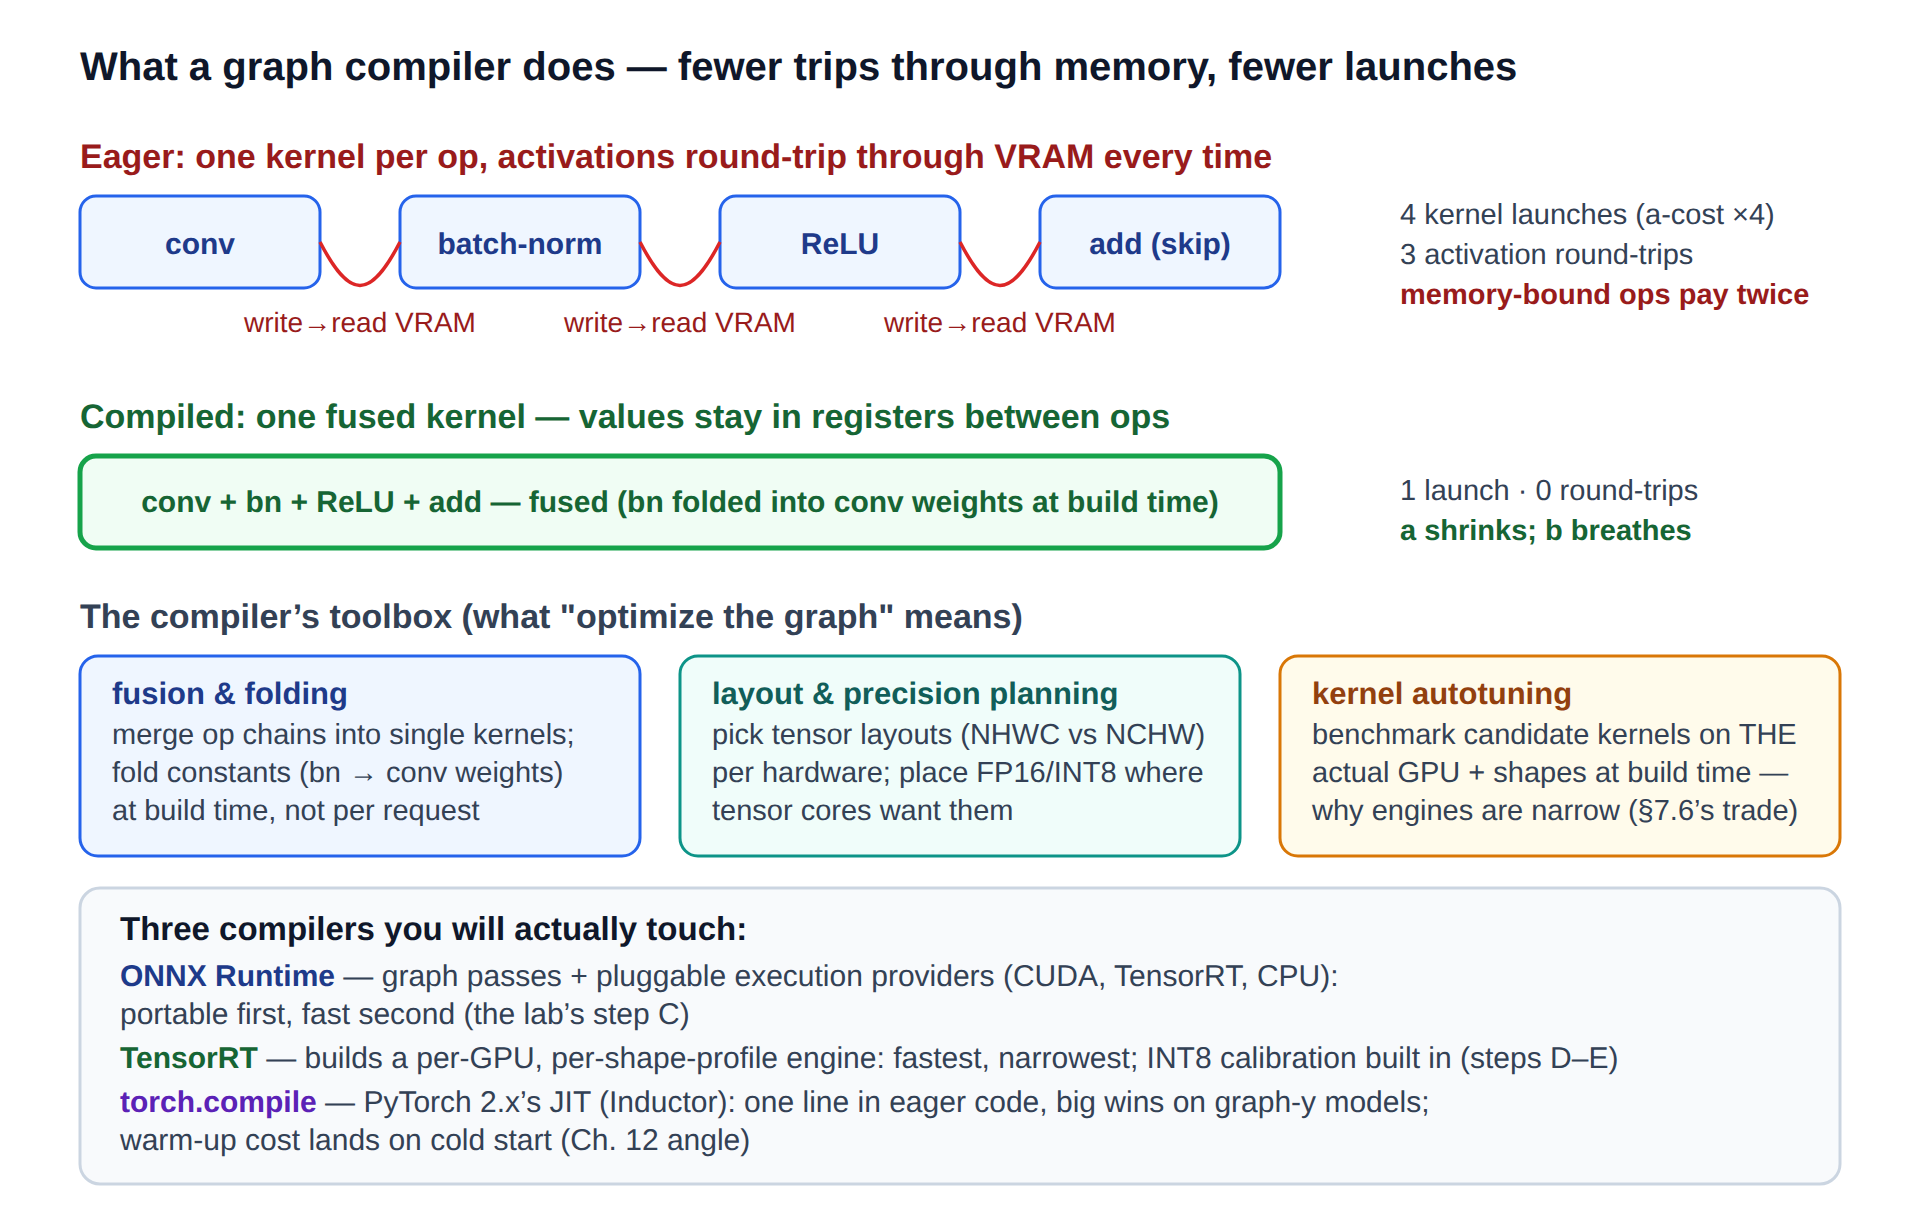
\includegraphics{figures/fig10-5_compiler.png}}\\[3pt]
  \figcaption{Figure 10-5  What a compiler does. Eager: one kernel per op, activations round-tripping through memory. Compiled: fused kernels, values staying in registers — a shrinks, and the memory wall is paid once instead of thrice.}
\end{tbbfigure}

\subsection*{The toolbox: what "optimize the graph" actually means}

Hand a compiler the whole graph (§7.6's exported artifact — this is why export formats exist) and four families of rewrites become possible. \textbf{Fusion}: merge chains of elementwise and normalization ops into their producer's kernel, so conv+bn+ReLU+add becomes \textit{one} launch whose intermediate values never leave registers — one trip through the wall instead of four launches and three round-trips. \textbf{Constant folding}: anything computable at build time is computed at build time — batch-norm's scale and shift fold into the conv's weights (they are just constants once training ends), reshapes collapse, dead branches vanish. \textbf{Layout and precision planning}: tensor cores want specific memory layouts (NHWC vs. NCHW) and precisions in specific places; the compiler re-lays tensors once, globally, instead of transposing per-op. \textbf{Kernel autotuning}: for each fused op there are dozens of candidate implementations (tilings, unrollings, tensor-core paths); the compiler \textit{benchmarks them on your actual GPU with your actual shapes} at build time and bakes the winners in. That last item is both the biggest single win and the source of the trade you already know from §7.6: \textbf{the output is married to one GPU model and one shape envelope} — fastest, narrowest.

\subsection*{Count it yourself: where 8.4 → 3.1 ms actually went}

"The compiler shrank a" should not stay a slogan when you can account for it on one napkin. A ResNet-class classifier runs roughly \textbf{175 CUDA operations} per eager forward pass (≈53 convs, their batch-norms, \textasciitilde{}49 ReLUs, 16 residual adds, plus pooling and the head). In eager mode each one pays Python dispatch plus a kernel launch — call it \textbf{\textasciitilde{}25 μs of overhead per op} — so the pass carries 175 × 25 μs ≈ \textbf{4.4 ms of pure administration}, work the GPU never sees. TensorRT fuses those 175 ops into \textbf{\textasciitilde{}60 kernels}, executed from C++ with no per-op Python: overhead falls to \textasciitilde{}0.3 ms. Add the memory-wall share: batch-1 intermediate activations total \textasciitilde{}45 MB, and eager's separate bn/ReLU/add kernels re-read and re-write them for roughly \textbf{90 MB of avoidable traffic ≈ 0.3 ms} at 320 GB/s. Administration (≈4.1 ms saved) + round-trips (≈0.3 ms) + a few dozen ops that constant folding deleted outright ≈ \textbf{the 5.3 ms that vanished from a}. The accounting also predicts a subtlety you can check in Transcript 10-6: at batch 32 those activations are 32× larger (\textasciitilde{}3 GB of avoidable traffic ≈ 9 ms per pass, \textasciitilde{}0.3 ms \textit{per item}) — so fusion quietly nibbles b too, which is exactly the small b-dip the fit shows from C to D (1.74 → 1.62 ms).

And here is constant folding's party trick in full, because it is three lines of algebra that delete an entire operator class from your network. Batch-norm at inference applies y = γ·(z − μ)/σ + β to the conv output z = Wx + b, with all four parameters \textbf{frozen constants} once training ends. Substitute and regroup: \textbf{y = (γ/σ)·W·x + (γ(b − μ)/σ + β)} — which is just another convolution, with weights W′ = (γ/σ)W and bias b′ = γ(b − μ)/σ + β, computable \textit{at build time}. Fifty-three batch-norms → zero batch-norms, before fusion even starts. (This is also a quiet warning for §7.6's equivalence battery: the folded network is algebraically identical but floating-point \textit{re-associated} — bit-identity is gone the moment the compiler touches it, which is why the battery tests tolerances, not bits.)

\subsection*{Three compilers, one decision pattern}

\textbf{ONNX Runtime} is the portable middle: it applies graph passes (fusion, folding) and then dispatches to a pluggable \textbf{execution provider} — CUDA, TensorRT, CPU, others — so one artifact serves everywhere at a good-not-maximal speed; it was Exhibit 10-A's free 1.4× (row C), and it is the sane default when your fleet is heterogeneous. \textbf{TensorRT} goes all in on NVIDIA: its \textit{builder} consumes the graph plus an \textbf{optimization profile} (the shape ranges you promise to send: min/opt/max batch and dimensions), autotunes per-layer kernels for the exact GPU, optionally calibrates INT8 (§10.3's scales, computed by the same builder), and emits an \textbf{engine} — a serialized plan that loads fast and runs fastest (rows D–E). The engine's narrowness is operational, not theoretical: it will refuse shapes outside its profile and will not run on a different GPU generation, which is why the lab labels artifacts \code{t4/\allowbreak clf\_int8.plan} (Chapter 4's digest discipline, extended with a hardware coordinate). \textbf{torch.compile} (PyTorch 2.x) is the eager-native path: one decorator captures graphs from ordinary Python and JIT-compiles them (Inductor) — big wins for graph-y models with almost no workflow change; its costs land differently: compilation happens at \textit{runtime}, so the first requests pay a warm-up that your readiness probe and cold-start budget must absorb (Chapters 5 and 12 have opinions), and dynamic control flow can fragment the graph into many small compilations.

\begin{terminalbox}
\begin{Verbatim}[breaklines=true,breakanywhere=true,fontsize=\small,formatcom=\color{tbbtermfg},codes=\tbbcodeactive]
# the lab's two builds, in full (CI steps - never at pod start):
$ trtexec --onnx=clf.onnx --saveEngine=t4/clf_fp16.plan --fp16 \
          --minShapes=input:1x3x224x224 \
          --optShapes=input:16x3x224x224 \
          --maxShapes=input:32x3x224x224    # the shape PROMISE
$ trtexec --onnx=clf.onnx --saveEngine=t4/clf_int8.plan --int8 \
          --calib=calib.cache               # §10.3, inside the builder
# engines are per-GPU, per-profile: the t4/ prefix is load-bearing.
# send a 64-batch to a max=32 engine -> refused. the narrowness is real.
\end{Verbatim}
\end{terminalbox}
\figcaption{Transcript 10-4  Building TensorRT engines. The optimization profile is a promise about shapes; INT8 calibration runs inside the builder; and the artifact path carries the GPU coordinate — because the engine will not survive without it.}

\begin{tbbtablewrap}
  \begin{tabular}{@{}>{\raggedright\arraybackslash}m{\dimexpr 0.1862\tbltextwidth-2\tabcolsep\relax} >{\raggedright\arraybackslash}m{\dimexpr 0.2128\tbltextwidth-2\tabcolsep\relax} >{\raggedright\arraybackslash}m{\dimexpr 0.2021\tbltextwidth-2\tabcolsep\relax} >{\raggedright\arraybackslash}m{\dimexpr 0.1862\tbltextwidth-2\tabcolsep\relax} >{\raggedright\arraybackslash}m{\dimexpr 0.2128\tbltextwidth-2\tabcolsep\relax}@{}}
  \arrayrulecolor{tbbnavy}\specialrule{1pt}{0pt}{0pt}
  \rowcolor{tbbtablehead}{\centering \bfseries\color{tbbnavy}Tool} & {\centering \bfseries\color{tbbnavy}Compiles when} & {\centering \bfseries\color{tbbnavy}Artifact \& scope} & {\centering \bfseries\color{tbbnavy}Exhibit 10-A win} & {\centering \bfseries\color{tbbnavy}The bill it sends} \\
  \arrayrulecolor{tbbnavy}\specialrule{0.7pt}{0pt}{2pt}
  {\textbf{ONNX Runtime}} & {Load time (graph passes) + EP dispatch} & {One .onnx, runs anywhere an EP exists} & {1.4× (row C)} & {Good-not-maximal speed; op-coverage edges} \\
  \arrayrulecolor{tbbtableborder}\hline
  {\textbf{TensorRT}} & {Build time, in CI (minutes per GPU-profile)} & {Engine married to one GPU + shape profile} & {1.6–2.0× (rows D–E)} & {Narrowness: per-GPU artifacts, refused shapes} \\
  \arrayrulecolor{tbbtableborder}\hline
  {\textbf{torch.compile}} & {Runtime, on first calls (JIT)} & {None — a decorator; cache is best-effort} & {(not benchmarked)} & {Warm-up on the cold-start path; recompiles on new shapes} \\
  \arrayrulecolor{tbbnavy}\specialrule{1pt}{2pt}{0pt}
  \end{tabular}\par
  \figcaption{Table 10-2  Three compilers at a glance — the row you pick is a workflow decision before it is a speed decision}
\end{tbbtablewrap}

\subsection*{torch.compile, timed — where the JIT bill actually lands}

The third row of Table 10-2 deserves a transcript of its own, because its trade is \textit{temporal} rather than spatial — you pay in \textit{when}, not in \textit{where} — and because it is the one your teammates will reach for first (it is one line). Watch the classifier:

\begin{terminalbox}
\begin{Verbatim}[breaklines=true,breakanywhere=true,fontsize=\small,formatcom=\color{tbbtermfg},codes=\tbbcodeactive]
>>> model_c = torch.compile(model)        # one line. too easy?
>>> t(model_c, batch=1)   # first call: Dynamo traces, Inductor
call 1:   38,400 ms       # autotunes kernels... on the SERVING pod
>>> t(model_c, batch=1)
steady:        6.1 ms     # vs eager 10.5 -> a real 1.7x. BUT:
>>> t(model_c, batch=7)   # a shape it has not seen ->
call 1:    9,200 ms       # recompile. every novel shape, again.
# the win is real and the bill is real: ~40 s on the cold-start path
# (Ch. 5's probes + Ch. 12's scale-out both notice), and dynamic
# shapes -> recompiles (mark_dynamic / bucketing, §10.5, tames it).
\end{Verbatim}
\end{terminalbox}
\figcaption{Transcript 10-5  torch.compile pays at runtime. Steady-state wins like a compiler; the first call (and every unseen shape) bills like one too — 38 s that lands squarely on the pod's readiness window, not in CI where TensorRT paid it.}

The operational reading: \textbf{TensorRT moved compilation into CI; torch.compile moved it onto your pod.} Neither is wrong — the second is unbeatable for iteration speed and models whose Python refuses to export — but the 38 seconds must live \textit{somewhere}, and the three respectable homes are: a \textbf{readiness-probe warm-up} that runs representative shapes before the pod reports Ready (Chapter 5's probe doing exactly what it was designed for); a \textbf{persistent compile cache} shipped in the image or a volume (best-effort — cache keys include GPU, versions, shapes); or \textbf{ahead-of-time export} (\code{torch.export} + AOTInductor — the ecosystem's current effort to give eager-native models a CI-built artifact, worth watching). What is \textit{not} respectable is discovering the bill during Week 12's autoscaling lab, when every scale-out pod spends its first 40 seconds compiling while the queue it was launched to absorb keeps growing — the retry-storm waveform from Chapter 9, self-inflicted.

\subsection*{When compilation disappoints — and the checklist that predicts it}

Compilation is not free speed everywhere, and the failure modes are predictable from this chapter's two ideas. If the model is \textbf{utterly memory-bound on weights} (batch-1 LLM decode), fusion of activation traffic barely moves the total — the weights dominate, and quantization, not compilation, owns that floor (§10.2's diagnosis, again first). If shapes are \textbf{wildly dynamic} (ragged text lengths, variable images), engines fragment across profiles and torch.compile recompiles — §10.5's bucketing is the answer \textit{before} the compiler. If the Python is \textbf{data-dependent}, the graph breaks: a single \code{if x.mean().item() > 0:} forces a GPU→CPU sync and splits the model into two graphs at that line; a Python loop over tokens becomes one compilation per iteration — \code{torch.compile} reports these (\code{fullgraph=True} turns them into errors worth reading). If the graph is \textbf{full of custom ops}, the compiler falls back per-op and fuses nothing — the export-coverage caveat from §7.6, now with a performance bill. And every compiled artifact adds \textbf{build-time and warm-up} to your pipeline: engines take minutes to build per GPU-profile pair (CI cost), torch.compile takes its toll on first requests (cold-start cost). The pattern for all four: know your side of the wall, know your shapes, and let the \textit{gate + sweep} — not the brochure — decide. (Numerically, compilers legitimately reorder float math; your §7.6 equivalence battery already covers this — run it per compiled artifact exactly as for quantized ones. Fused-and-reordered is still changed.)

\begin{calloutbox}{tbbpurple}{tbbpurplefill}
{\normalsize\bfseries\color{tbbpurple}Think About It}\par\vspace{3pt}
\begin{tbbitemize}
  \item Row C→D of Exhibit 10-A gained mostly in a (8.4→3.1 ms in Figure 10-6's fit) and barely in b. Explain, mechanism by mechanism, why fusion and autotuning land in a while INT8 lands in b — and what that predicts about which models benefit most from each.
  \item Your teammate torch.compiles the chat model and celebrates a 1.7× steady-state win — then the Week 12 autoscaler starts flapping and p99 spikes on every scale-out. Connect the two facts, name the two mitigations (one from Ch. 5, one from Ch. 12's toolbox), and say what you would measure to confirm.
  \item Design the CI matrix for a two-GPU fleet (T4 + A100) with FP16 and INT8 variants: how many engine builds, how many gate runs, and what does the model-store layout look like (Ch. 6 prefixes)? Where does a new GPU generation's arrival hurt?
\end{tbbitemize}
\end{calloutbox}

\section{Composing the Levers — Re-fitting a and b}

Chapter 9 promised that this week would "re-run exactly that sweep and re-fit exactly those two numbers." Here is the payment. Recall the law — \textbf{t(B) = a + b·B} — fitted on the Week 9 classifier at a = 8.4 ms, b = 2.05 ms. Two runs per variant (batch 1 and batch 32) re-fit it after each optimization, and the fit is a diagnosis: it tells you not just \textit{that} a variant is faster but \textbf{where the speed came from} — which is what separates a benchmark report from a bar chart.

\begin{terminalbox}
\begin{Verbatim}[breaklines=true,breakanywhere=true,fontsize=\small,formatcom=\color{tbbtermfg},codes=\tbbcodeactive]
# refit a,b from two timed points per variant (t1, t32):
$ python fit.py --t1 10.5 --t32 74.0     # B: eager FP16 (Wk 9)
  a = 8.4 ms    b = 2.05 ms    ceiling 1/b = 488/s
$ python fit.py --t1  7.6 --t32 61.6     # C: ONNX Runtime
  a = 5.9 ms    b = 1.74 ms    ceiling 575/s
$ python fit.py --t1  4.7 --t32 55.0     # D: TensorRT FP16
  a = 3.1 ms    b = 1.62 ms    ceiling 617/s
$ python fit.py --t1  3.8 --t32 32.3     # E: TensorRT INT8
  a = 2.9 ms    b = 0.92 ms    ceiling 1,087/s
# compilation attacked a (8.4->3.1): launches, round-trips, folding.
# quantization attacked b (2.05->0.92): the bytes per item.
# exactly as Chapter 9 predicted. write BOTH stories in the report.
\end{Verbatim}
\end{terminalbox}
\figcaption{Transcript 10-6  The re-fit. Each optimization signs its work: compilers shrink the fixed cost a, quantization shrinks the marginal cost b — and the ceiling 1/b more than doubles. Two runs per variant is all the fit needs.}

\begin{tbbfigure}
  \adjustbox{max width=0.94\linewidth,max totalheight=0.46\textheight}{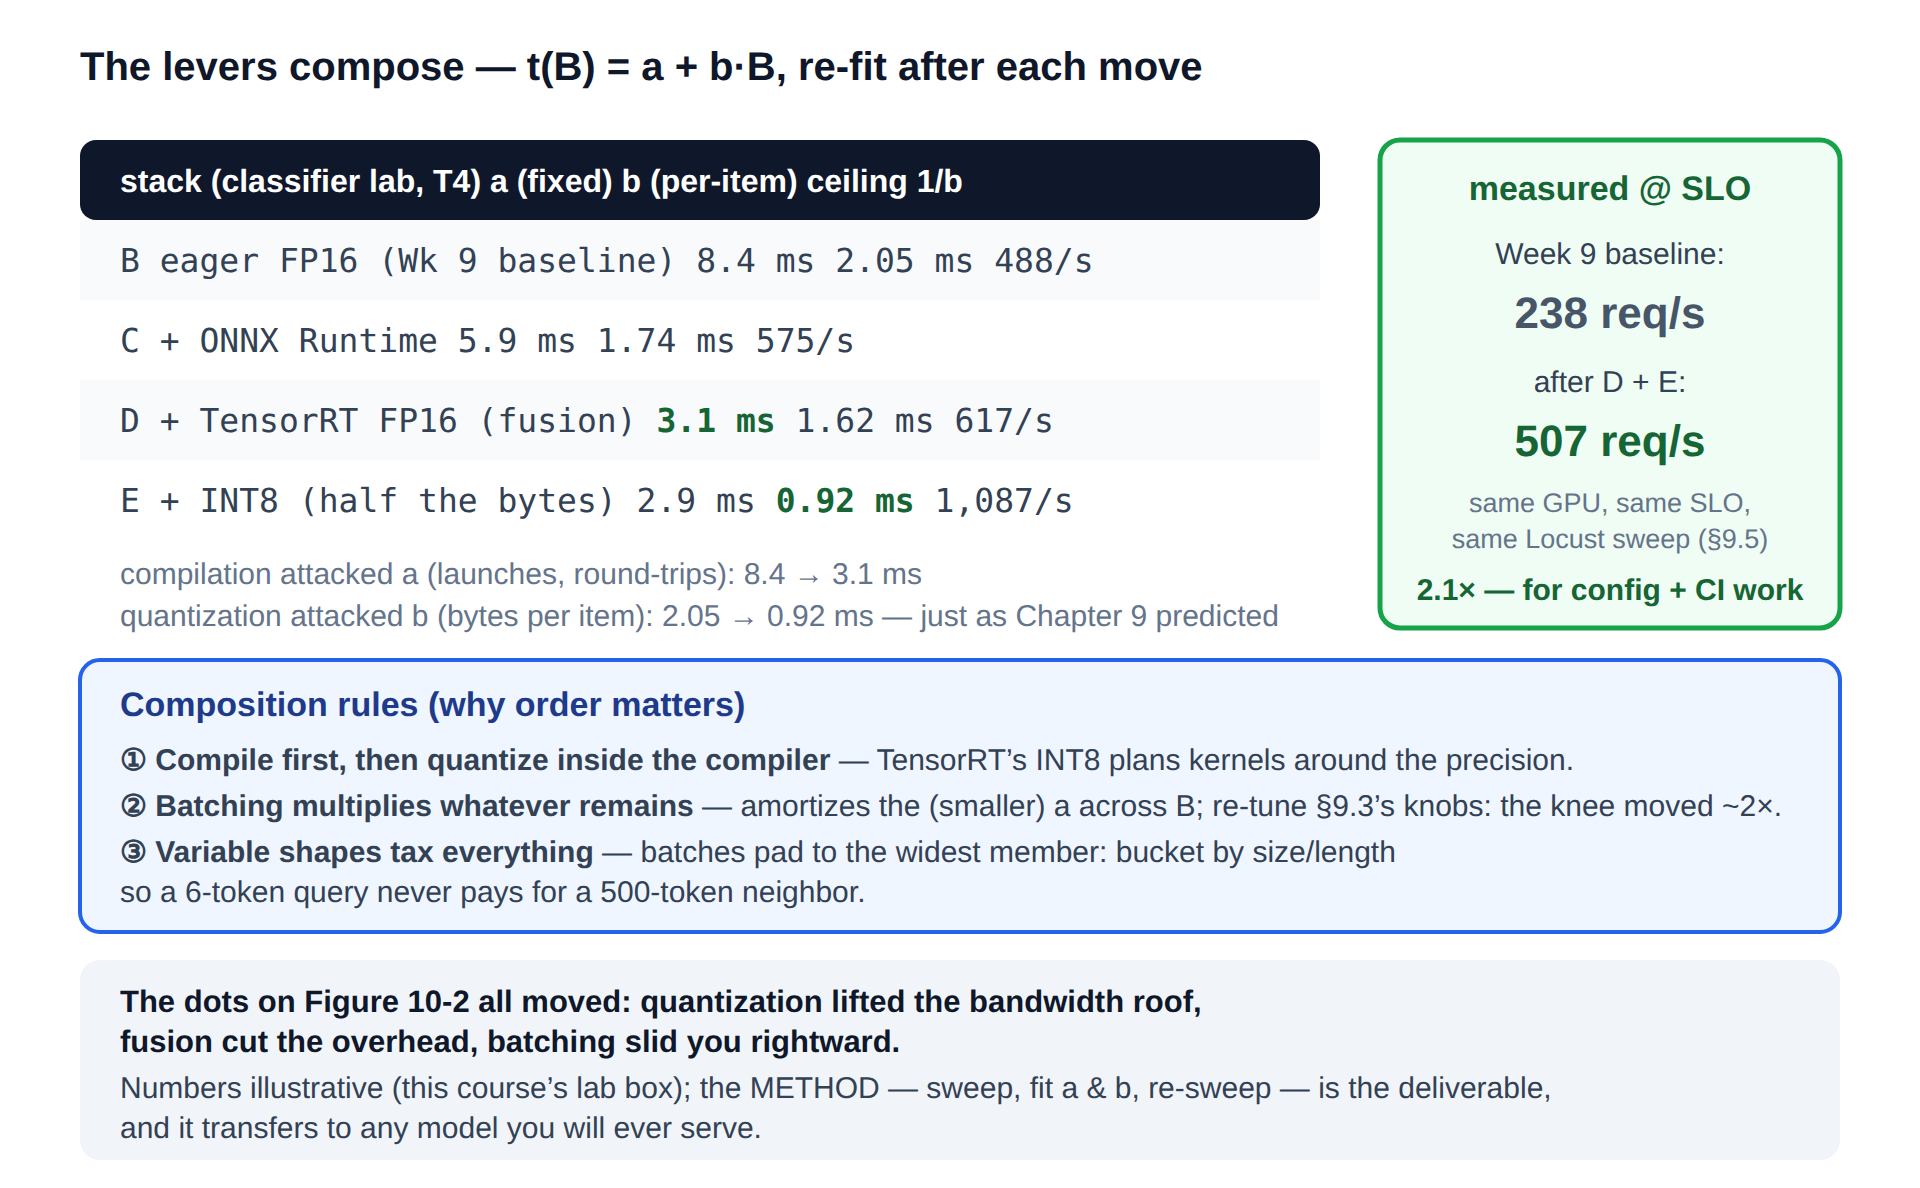
\includegraphics{figures/fig10-6_levers.png}}\\[3pt]
  \figcaption{Figure 10-6  The levers compose. The full a/b table, the measured @-SLO numbers (238 → 507 req/s), and the composition rules — order matters, and variable shapes tax everything.}
\end{tbbfigure}

\subsection*{Why batching works — the principle, stated once with algebra}

The syllabus calls this week's third topic "the principle of dynamic batching," and after two chapters of using it you have earned the one-line version: divide t(B) = a + b·B by B and you get the \textbf{cost per item, c(B) = b + a/B} — a hyperbola falling toward b. That is the entire principle. \textbf{Batching is a-amortization and nothing else}: it spreads the fixed cost (launches, scheduling, the weight stream) across B riders, it cannot touch b, and its returns diminish \textit{by arithmetic, not by folklore} — going from B to 2B recovers a/2B per item, so each doubling buys half as much as the last. Table 10-3 runs the numbers for the optimized classifier (a = 2.9, b = 0.92):

\begin{tbbtablewrap}
  \begin{tabular}{@{}>{\raggedright\arraybackslash}m{\dimexpr 0.1383\tbltextwidth-2\tabcolsep\relax} >{\raggedright\arraybackslash}m{\dimexpr 0.2128\tbltextwidth-2\tabcolsep\relax} >{\raggedright\arraybackslash}m{\dimexpr 0.2553\tbltextwidth-2\tabcolsep\relax} >{\raggedright\arraybackslash}m{\dimexpr 0.2021\tbltextwidth-2\tabcolsep\relax} >{\raggedright\arraybackslash}m{\dimexpr 0.1915\tbltextwidth-2\tabcolsep\relax}@{}}
  \arrayrulecolor{tbbnavy}\specialrule{1pt}{0pt}{0pt}
  \rowcolor{tbbtablehead}{\centering \bfseries\color{tbbnavy}Batch B} & {\centering \bfseries\color{tbbnavy}t(B) = a + b·B} & {\centering \bfseries\color{tbbnavy}Per item c(B) = b + a/B} & {\centering \bfseries\color{tbbnavy}Ideal req/s = B/t(B)} & {\centering \bfseries\color{tbbnavy}Of ceiling (1/b)} \\
  \arrayrulecolor{tbbnavy}\specialrule{0.7pt}{0pt}{2pt}
  {1} & {3.8 ms} & {3.82 ms} & {262/s} & {24\%} \\
  \arrayrulecolor{tbbtableborder}\hline
  {4} & {6.6 ms} & {1.65 ms} & {608/s} & {56\%} \\
  \arrayrulecolor{tbbtableborder}\hline
  {16} & {17.6 ms} & {1.10 ms} & {908/s} & {84\%} \\
  \arrayrulecolor{tbbtableborder}\hline
  {32} & {32.3 ms} & {1.01 ms} & {990/s} & {91\%} \\
  \arrayrulecolor{tbbtableborder}\hline
  {\textbf{∞}} & {—} & {\textbf{→ b = 0.92 ms}} & {\textbf{→ 1,087/s}} & {100\%} \\
  \arrayrulecolor{tbbnavy}\specialrule{1pt}{2pt}{0pt}
  \end{tabular}\par
  \figcaption{Table 10-3  Amortization, computed (INT8 variant: a = 2.9 ms, b = 0.92 ms). The knee is visible in the third column — and "ideal req/s" ignores queueing, so real @-SLO numbers sit below it (Ch. 7's headroom).}
\end{tbbtablewrap}

Two readings of the table pay for the algebra. First, \textbf{the word "dynamic" is the hard part, and it is a queueing word, not a GPU word}: traffic arrives one request at a time, so the §9.3 batcher buys amortization \textit{with waiting} — hold the first request up to max\_queue\_delay hoping for co-riders, subject to wait + t(B) fitting the SLO budget. The self-regulation you observed in Chapter 9 now has a mechanism: at low load the window expires nearly empty (small batches — fine, an idle system needs no efficiency), at high load it fills instantly (big batches — efficiency arriving exactly when demanded). Second, \textbf{optimization moved the knee, in a direction that should now be intuitive}: with a cut from 8.4 to 2.9 ms there is simply \textit{less fixed cost to amortize} — batch 4 already banks 56\% of the ceiling (it was \textasciitilde{}49\% pre-optimization), deeper batching buys thinner slices, and the correct response is often to \textit{shorten} the delay window and take the latency win. That is rule ② below, derived rather than asserted — and it is why "re-tune the knobs after optimizing" is not optional hygiene but the same two constants, moved.

\subsection*{The composition rules}

Three rules govern how the levers stack, and each is a mistake someone in your cohort will otherwise make. \textbf{Rule ① — compile first, quantize inside the compiler.} TensorRT's INT8 mode plans kernels \textit{around} the precision (which layers, which fused groups, where the dequant boundaries sit); quantizing a graph the compiler never sees leaves both tools working blind — this is why row E of Exhibit 10-A was "TensorRT INT8," one build, not two bolt-ons. \textbf{Rule ② — batching multiplies whatever remains.} The batcher amortizes the now-smaller a across B items, so the §9.3 knobs need re-tuning after optimization: with a = 2.9 ms instead of 8.4, smaller batches reach efficiency sooner, the knee sits \textasciitilde{}2× further out, and your max\_queue\_delay can often \textit{shrink} while throughput still rises — re-sweep, don't assume. \textbf{Rule ③ — variable shapes tax everything.} A batch pads every member to the widest; a 6-token query co-batched with a 500-token document pays for 500 tokens of work. The remedy is \textbf{bucketing} — group requests by size class (image resolutions, sequence-length bands) so padding waste stays bounded — and it must be designed \textit{with} the compiler's shape profiles (§10.4): buckets and profiles are the same decision seen from two tools. (Week 11 pushes this to its logical end: continuous batching exists because LLM generation makes every sequence a different length every step.)

One honest footnote the report must carry: these gains are \textbf{per-replica economics, not magic}. The 507 req/s variant still obeys the hockey stick (the knee just moved), still needs headroom for its SLO, and still fails the gate if the calibration was lazy. And the composed win is what re-prices the fleet: the project model's 28 → 57 req/s at the SLO is exactly the 8-replica → 4-replica, \$4,762 → \$2,381 move Chapter 7 promised — with Week 12's autoscaling still waiting to halve the bill again.

\begin{calloutbox}{tbbpurple}{tbbxF5F3FF}
{\normalsize\bfseries\color{tbbx5B21B6}Box 10-2  The rest of the menu — levers this week deliberately did not pull}\par\vspace{3pt}
This chapter's three levers share one property: \textbf{no training loop required} — they run in CI, in minutes, on the artifact you already have. The wider menu trades that away for bigger or different wins. Know it exists, and know the price tag:

\begin{tbbitemize}
  \item \textbf{Distillation} (Hinton et al., 2015): train a small \textit{student} to imitate a large \textit{teacher}'s outputs — DistilBERT famously kept \textasciitilde{}97\% of BERT's capability at 40\% fewer parameters. The win is architectural and permanent; the price is a full training pipeline, data, and weeks — a \textit{modeling} project, not a CI step.
  \item \textbf{Pruning \& structured sparsity}: delete weights outright. Unstructured pruning rarely pays on GPUs (irregular zeros don't skip work); \textbf{2:4 structured sparsity} (two zeros per four weights, Ampere+ tensor cores) genuinely doubles the math rate — after a sparsify-and-fine-tune cycle that, again, is training.
  \item \textbf{Speculative decoding} (Week 11): a small model drafts tokens, the big model verifies them in one batched pass — attacking the LLM's per-token weight-stream directly. Needs no retraining, but it is generation-specific machinery; it waits for the chapter where generation is the whole problem.
  \item \textbf{Cascades \& early exit}: route easy inputs to a small model, hard ones to the big one — a \textit{systems} lever (Chapter 12's router territory) whose gate is a routing metric, not an accuracy delta.
\end{tbbitemize}

The discipline is unchanged everywhere on the menu: diagnose first (§10.2), gate honestly (§10.3), attribute the win (§10.5). Only the currencies differ.
\end{calloutbox}

\vspace{3.0pt}

\begin{calloutbox}{tbbpurple}{tbbpurplefill}
{\normalsize\bfseries\color{tbbpurple}Think About It}\par\vspace{3pt}
\begin{tbbitemize}
  \item A teammate reports "INT8 gave us 1.26× at batch 32 — disappointing, the brochure said 2×." Using Transcript 10-6's numbers, show why the batch-32 speedup understates the @-SLO win (hint: compute t(32) ratios vs. ceiling ratios), and which single number they should have reported instead.
  \item After optimization, the old max\_queue\_delay=10 ms window now gathers batches that saturate past the SLO knee. Walk through re-tuning both §9.3 knobs with a = 2.9, b = 0.92, SLO 500 ms — what changes, what doesn't, and why must the memory.max from Ch. 5 be re-measured too?
  \item Your text service sees lengths 5–800 tokens, uniformly. Design the buckets (how many, what boundaries) and the matching TensorRT profiles — then compute the worst-case padding waste with and without them.
\end{tbbitemize}
\end{calloutbox}

\section{Lab: The Before/After Benchmark Report}

The lab is the chapter, executed on your own model — and its deliverable is the \textbf{before/after benchmark report} that the project rubric has required since Week 1 ("a before/after optimization comparison"). The shape (Figure 10-7): your Week 9 sweep is already the \textit{before}; this week builds gated variants, re-runs the identical sweep, and writes the two paragraphs that make a table into a report.

\begin{tbbfigure}
  \adjustbox{max width=0.94\linewidth,max totalheight=0.46\textheight}{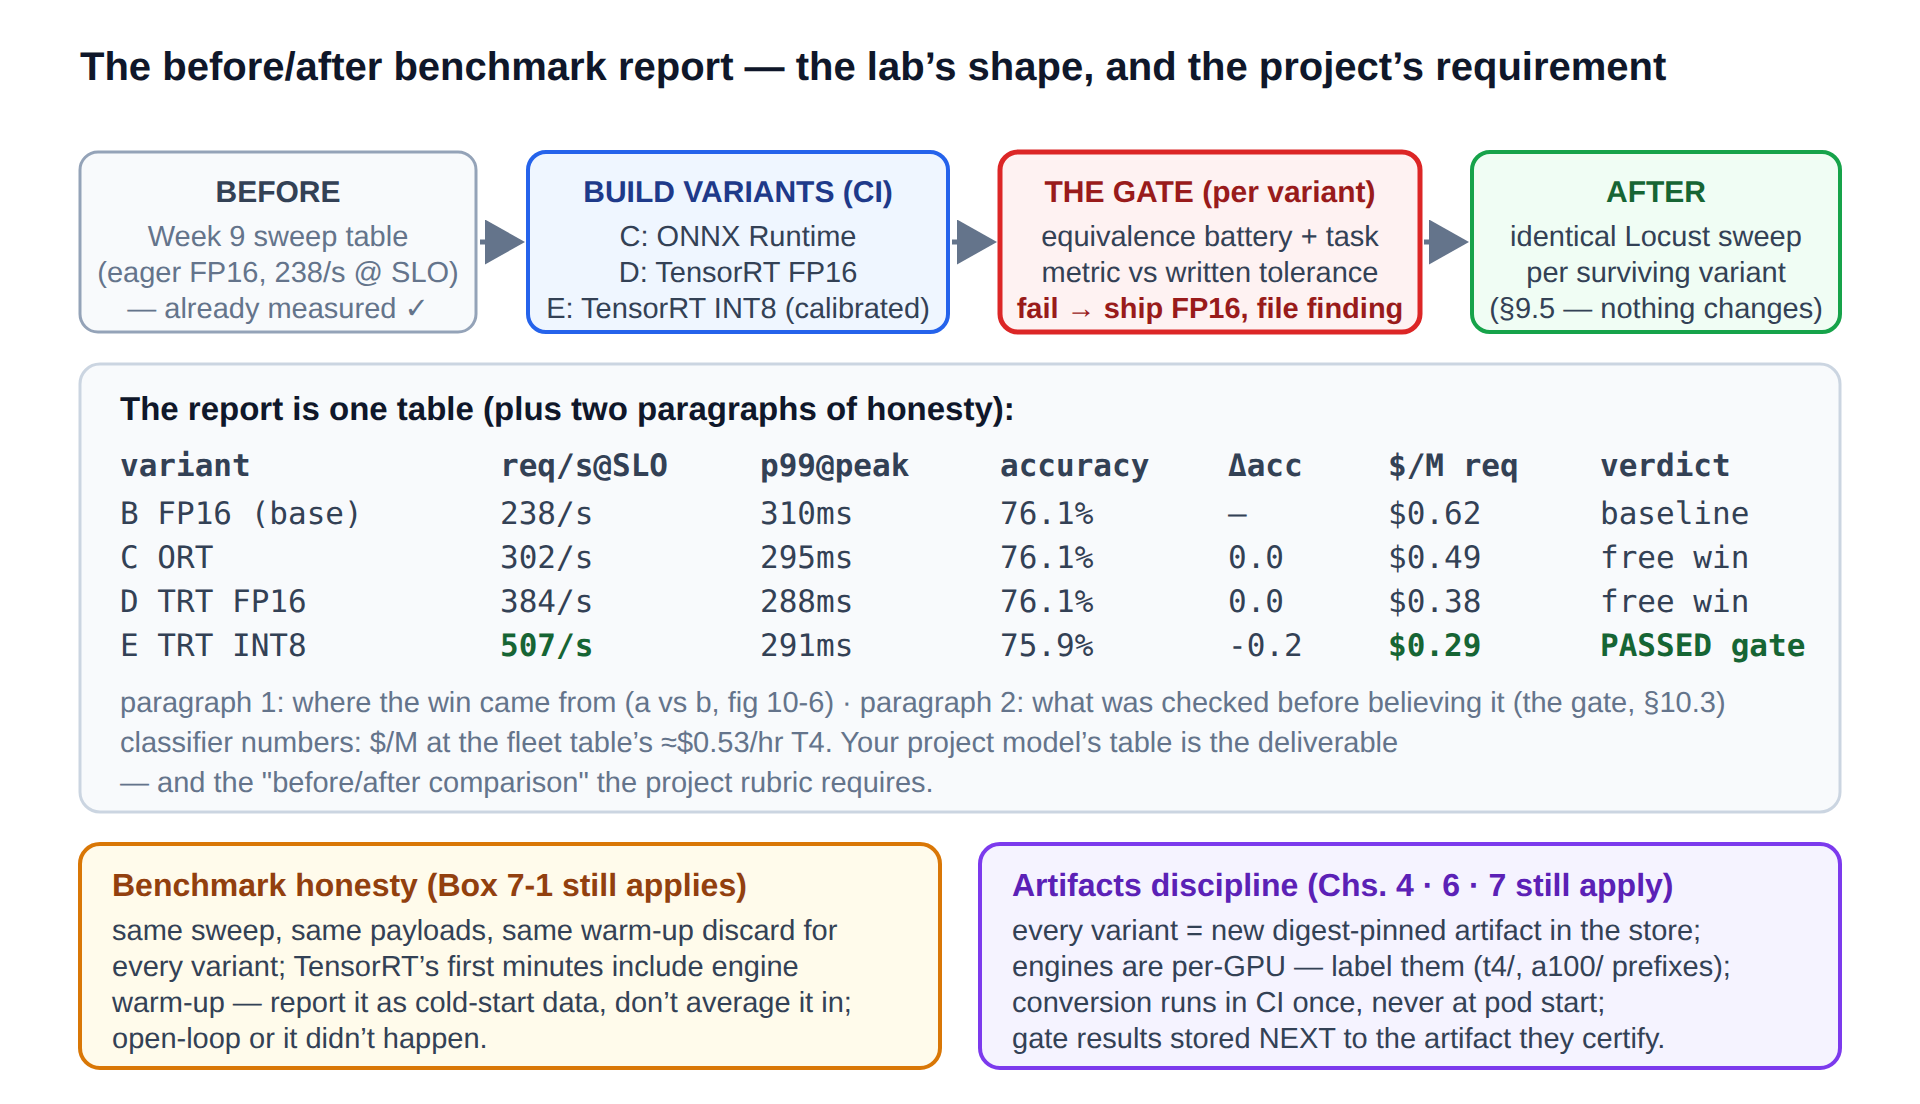
\includegraphics{figures/fig10-7_lab.png}}\\[3pt]
  \figcaption{Figure 10-7  The lab's pipeline and the report's anatomy: variants built in CI, each through the gate, each through the identical sweep — one table, two paragraphs of honesty.}
\end{tbbfigure}

\subsection*{The seven steps}

\begin{tbbitemize}
  \item \textbf{① Diagnose (§10.2).} Transcript 10-1's two lines for your model on your GPU: which side of the wall? Write the prediction — which lever should pay most — \textit{before} any build. (Being wrong here, visibly, is worth marks: it means the report taught you something.)
  \item \textbf{② Build variant C (§10.4).} Export → ONNX Runtime with the CUDA EP. Run §7.6's equivalence battery (this one should pass near-exactly).
  \item \textbf{③ Build variants D and E (§10.4 + §10.3).} TensorRT FP16 with explicit shape profiles; then INT8 with a curated calibration set — 500–1,000 inputs, stratified across classes \textit{and across the slices your gate checks}, drawn from recent traffic. Store the set's manifest (and its digest) next to the calib cache: the gate's credibility is exactly the calibration set's documentation.
  \item \textbf{④ Gate each variant (§10.3).} Task metric vs. the tolerance you wrote down first; slice checks; store each gate report beside its artifact. A failed gate ships FP16 and files the finding — that is a \textit{complete, passing} lab outcome.
  \item \textbf{⑤ Sweep each survivor (§9.5, unchanged).} Same locustfile, same rates, same warm-up discard. TensorRT's engine warm-up is reported as cold-start data, not averaged into steady state.
  \item \textbf{⑥ Re-fit a and b (§10.5).} Two extra timed points per variant; attribute every win to its mechanism. If the attribution surprises you, say so — that sentence is the most valuable one in the report.
  \item \textbf{⑦ Re-price (Ch. 7's bill).} New per-replica @-SLO number → new fleet size → new monthly cost, in the proposal. The project's cost narrative should now read: estimated → measured (Wk 9) → optimized (Wk 10), with Week 12's autoscaling as the declared next lever.
\end{tbbitemize}

What do "two paragraphs of honesty" actually sound like? Here is a model, written for the classifier so every number is one you have already met — copy its \textit{shape}, not its sentences:

\begin{calloutbox}{tbbteal}{tbbxF0FDFA}
{\normalsize\bfseries\color{tbbx115E59}Exhibit 10-B  The report's two paragraphs, written out}\par\vspace{3pt}
\textbf{¶1 — Where the win came from.} "Optimization moved the classifier from 238 to 507 req/s at the p99 ≤ 500 ms SLO (2.1×), or \$0.62 → \$0.29 per million requests on the T4. The re-fit attributes the gain: compilation cut a from 8.4 to 3.1 ms (dispatch and launch overhead — \textasciitilde{}175 eager ops fused to \textasciitilde{}60 kernels, §10.4's accounting) and trimmed b from 2.05 to 1.62 ms (fused activation round-trips); INT8 then cut b to 0.92 ms (the doubled tensor-core rate). Our step-① prediction was half right: we expected INT8's byte-halving to dominate, but the fit shows this model was \textit{launch-bound} at batch 1 and compute-leaning at batch 16 — the INT8 win came from math rate, not bytes. We were wrong about the mechanism and right about the magnitude; the distinction matters for the next model, which is 60× larger."

\textbf{¶2 — What was checked before believing it.} "Every variant passed §7.6's equivalence battery. INT8 passed the gate at −0.22 pt against the 0.5 pt tolerance recorded in the proposal \textit{before} benchmarking (report stored at t4/clf\_int8/gate.json). The slice check flagged \textit{streetcar} at −1.8 pt; the calibration manifest showed only 3 streetcar images, so we re-calibrated with 40 — the slice recovered to −0.6 pt with the global delta unchanged. All variants ran the identical locustfile (digest 9f3c…), identical rates, first 60 s discarded; TensorRT's engine load is reported under cold start, not averaged into steady state. Engines carry the t4/ prefix; the one A10G in the team refuses them, as designed."

\textit{Why this earns its grade: every number in ¶1 is attributed to a mechanism, every claim in ¶2 is checkable from a stored artifact — and the one wrong prediction is stated, not hidden. Graders (and future teammates, and Week 14's incident reviewer) read for exactly this.}
\end{calloutbox}

\vspace{3.0pt}

\begin{calloutbox}{tbbred}{tbbxFEF2F2}
{\normalsize\bfseries\color{tbbx991B1B}Box 10-1  Report red flags (the graders' checklist, published)}\par\vspace{3pt}
\begin{tbbitemize}
  \item \textbf{A speedup without a gate result} next to it — a fast wrong model is not an optimization.
  \item \textbf{Different sweeps for different variants} (rates, payloads, warm-up) — the comparison is the product; protect it.
  \item \textbf{Batch-N latency ratios presented as "the speedup"} — the number that matters is req/s at the SLO (goodput), plus the a/b attribution.
  \item \textbf{An engine artifact without a GPU coordinate} in its path/metadata — it WILL be deployed on the wrong fleet eventually (Ch. 4's digest lesson, hardware edition).
  \item \textbf{"We quantized in the pod at startup"} — conversion is CI, once, gated (§7.6, §10.4). The cold-start path stays sacred.
\end{tbbitemize}
\end{calloutbox}

\vspace{3.0pt}

Deliverables: the one-table report with its two paragraphs (where the win came from; what was checked before believing it), the gate outputs per variant, the re-fit constants, the updated proposal cost line — and the billing screenshot (the ritual survives; typical lab spend: \textasciitilde{}\$3–4 of T4 time, engine builds included).

\begin{calloutbox}{tbbpurple}{tbbpurplefill}
{\normalsize\bfseries\color{tbbpurple}Think About It}\par\vspace{3pt}
\begin{tbbitemize}
  \item Write your report's paragraph 1 in advance as a hypothesis ("we expect compilation to dominate because §10.2 says..."), then grade it after step ⑥. Which side of the wall was your model actually on?
  \item Your INT8 variant fails the gate by 0.9 pt against a 0.5 pt tolerance. List your four options in order of increasing cost (better calibration → per-channel/group granularity → weight-only/mixed precision → QAT), and the evidence that would justify escalating past each.
  \item The optimized model changes the Ch. 2 fleet answer: at 507 req/s per T4, is there ANY load at which the A100 (≈5× the price, ≈2.5× this model's throughput) wins for serving this classifier? Show the arithmetic — and name the workload where the A100 answer flips (hint: §10.2's wall).
\end{tbbitemize}
\end{calloutbox}

\namedsection{Summary}{The Chapter in Fifteen Points}

\qitem{1}{\textbf{Optimization means cost per request at the same SLO.} Exhibit 10-A: one model, one GPU, four stacks — 28 → 57 req/s at the same p99, \$7.94 → \$3.90 per million, and the fleet Chapter 7 promised: 8 replicas → 4, \$4,762 → \$2,381/month. Nothing about the model's knowledge changed.}

\qitem{2}{\textbf{You have trusted lossy compression your whole life} — 8-bit μ-law telephony (1962), JPEG (1992), MP3 (1993): find what the consumer of the signal needs, stop paying for the rest. Quantization applies the pattern with the model's own decision as the consumer — training needs fine ticks (tiny gradient steps), inference only needs the argmax/token to survive rounding, and flat minima make it survive.}

\qitem{3}{\textbf{The memory wall is the master diagnosis:} a T4 does 65 TFLOPS but moves 320 GB/s — \textasciitilde{}200 FLOPs must arrive per byte. Arithmetic intensity (FLOPs/byte) against that ridge decides everything; most serving-batch inference is memory-bound, so bytes, not math, are the bill (Transcript 10-1: two lines, no profiler).}

\qitem{4}{\textbf{On the roofline, each lever has a geometric meaning:} batching slides you right (weights re-used across B), quantization lifts the bandwidth roof (fewer bytes per weight), compilation stops paying the wall twice (fused kernels keep activations out of VRAM). And the ridge varies per card (Table 10-1): the L4 sits near 400, the A100's premium is mostly bandwidth — the wall grows taller every generation, so bytes are the appreciating currency.}

\qitem{5}{\textbf{The bytes take a three-speed journey (Ch. 6's promise, paid):} object store → host page cache (once per pod) → pinned H2D over PCIe (\textasciitilde{}12 GB/s, once per process) → VRAM to compute (300 GB/s, every pass). PCIe is \textasciitilde{}25× slower than VRAM and pageable copies halve it again — so weights cross once at startup, per-request tensors get pinned buffers and async copies, and nvidia-smi dmon's PCIe columns are the diagnosis's third line.}

\qitem{6}{\textbf{Floats forgive, integers delegate:} a float re-scales itself per value (the exponent); an integer shares one calibrated scale per tensor — the root of every §10.3 gotcha. FP16 trades range (loss-scaling in training), BF16 keeps FP32's range and won training, FP8 (Hopper/Ada) is integer-cost storage with self-scaling left in — and INT8×INT8 sums accumulate in INT32, so bad accuracy is always tick placement, never overflow.}

\qitem{7}{\textbf{Quantization = a coarser ruler placed well:} q = round(w/scale) + zero\_point (asymmetric zero\_point slides the ruler so post-ReLU ranges waste no ticks); per-channel scales for weights — one shared scale costs a ±0.05 channel 21\% error, its own ruler 0.4\% (per-group for INT4 LLMs); calibration picks activation ranges via min–max, percentile, or KL — its quality IS the quantization's quality. PTQ is minutes in CI; QAT is the escalation when PTQ fails the gate.}

\qitem{8}{\textbf{The two gotchas:} ranges differ per channel (hence per-channel scales), and transformer activations hide outliers (LLM.int8(), 2022) — hence weight-only quantization as the LLM default, smoothing, or mixed precision. CNN-class lab models tolerate full W8A8.}

\qitem{9}{\textbf{The gate makes lossy legal:} task metric (not vibes) vs. a tolerance written BEFORE the benchmark, plus slice checks — and the output is a NEW digest-pinned artifact with its gate report beside it. Failing the gate and shipping FP16 is a passing outcome; shipping ungated is how "the model got weird" tickets are born.}

\qitem{10}{\textbf{Compilers buy a: fusion, folding, layout planning, autotuning} — one launch instead of four, zero activation round-trips, kernels benchmarked on your exact GPU and shapes at build time. The price is narrowness: engines are per-GPU, per-shape-profile (t4/ prefixes are load-bearing), and torch.compile's warm-up lands on the cold-start path.}

\qitem{11}{\textbf{Three compilers, one pattern:} ONNX Runtime (portable middle, pluggable EPs), TensorRT (fastest, narrowest, INT8 calibration in the builder), torch.compile (eager-native, runtime JIT). Compilation disappoints predictably: weight-bound decode, wild shapes, custom ops — diagnose first.}

\qitem{12}{\textbf{Batching is a-amortization, nothing else:} c(B) = t(B)/B = b + a/B — a hyperbola falling toward b, where each doubling of B buys half what the last one did; the knee is arithmetic, not folklore (Table 10-3: batch 4 already banks 56\% of the optimized ceiling). \textit{Dynamic} is the queueing half: trade bounded waiting for co-riders inside the SLO budget, self-regulating with load.}

\qitem{13}{\textbf{Composition rules:} compile first and quantize inside the compiler; batching multiplies whatever remains (re-tune §9.3's knobs — the knee moved, and with less a to amortize the delay window can often \textit{shrink}); variable shapes tax everything (bucket by size, co-designed with shape profiles).}

\qitem{14}{\textbf{The re-fit is the report:} t(B) = a + b·B, two runs per variant — compilation signs its work in a (8.4 → 3.1 ms), quantization in b (2.05 → 0.92 ms), ceiling 488 → 1,087/s, measured 238 → 507 req/s @ SLO. Attribution turns a bar chart into engineering.}

\qitem{15}{\textbf{Optimization re-prices hardware:} the 70B poster child drops 140 → \textasciitilde{}35 GB at INT4; models that needed A100s fit T4 fleets; Chapter 2's table and Chapter 5's nodeSelector get new right answers. Re-read the fleet table after every precision change.}

\namedsection{Exercises}{}

\subsection*{A. Multiple choice}

\qitem{1}{A 7B model in FP16 (14 GB of weights) generates tokens at batch 1 on a GPU with 700 GB/s bandwidth. Which is the best estimate of the per-token latency floor, and its cause?}

\begin{tbboptions}
  \item ① \textasciitilde{}2 ms — kernel launch overhead        ② \textasciitilde{}20 ms — weights must stream once per token (14 GB ÷ 700 GB/s)
  \item ③ \textasciitilde{}0.1 ms — the math is trivial        ④ It cannot be estimated without a profiler
\end{tbboptions}

\qitem{2}{Which change does quantizing weights from FP16 to INT8 NOT directly produce?}

\begin{tbboptions}
  \item ① Half the bytes streamed per pass        ② Half the VRAM for weights
  \item ③ Double the tensor-core arithmetic rate (on INT8-capable GPUs)        ④ Better model accuracy
\end{tbboptions}

\qitem{3}{Transformer activation outliers break naive W8A8 quantization because:}

\begin{tbboptions}
  \item ① INT8 cannot represent negative numbers
  \item ② A few huge values stretch the scale so ordinary values round to almost nothing
  \item ③ Activations change every request, so no scale can exist
  \item ④ GPUs process activations in FP64
\end{tbboptions}

\qitem{4}{The correct order of operations for maximum benefit is:}

\begin{tbboptions}
  \item ① Quantize the ONNX file, then hand it to TensorRT        ② Build the TensorRT engine with INT8 mode + calibration, so the compiler plans kernels around the precision
  \item ③ Order is irrelevant; the gains are independent        ④ Batch first, then compile, then quantize at pod startup
\end{tbboptions}

\qitem{5}{Your re-fit shows variant X moved a from 8.4 → 3.2 ms with b unchanged. Variant X is most likely:}

\begin{tbboptions}
  \item ① INT8 quantization        ② Graph compilation (fusion + autotuning)
  \item ③ A bigger batch size        ④ A faster tokenizer
\end{tbboptions}

\qitem{6}{A TensorRT engine built with maxShapes batch=32 on a T4 receives a batch of 48 on an A10G. What happens?}

\begin{tbboptions}
  \item ① It runs, slightly slower        ② It silently truncates the batch
  \item ③ It fails twice over: wrong GPU for the engine, and shape outside the profile — engines are per-GPU, per-profile artifacts
  \item ④ TensorRT rebuilds the engine on the fly
\end{tbboptions}

\qitem{7}{The gate's tolerance ("≤ 0.5 pt top-1 loss") must be written before benchmarking because:}

\begin{tbboptions}
  \item ① Regulations require it        ② Otherwise the observed loss defines what is "acceptable" after the fact — the accuracy analog of promising an SLO before measuring (§7.4)
  \item ③ TensorRT needs it as a build flag        ④ It makes the report shorter
\end{tbboptions}

\qitem{8}{After optimization (a: 8.4→2.9, b: 2.05→0.92), which statement about the §9.3 batching knobs is correct?}

\begin{tbboptions}
  \item ① They are unaffected; batching is orthogonal
  \item ② The knee moved \textasciitilde{}2× outward, smaller batches reach efficiency sooner, and both knobs deserve a re-sweep — as does Ch. 5's memory.max
  \item ③ max\_queue\_delay must double        ④ max\_batch\_size no longer has a VRAM bound
\end{tbboptions}

\subsection*{B. Short answer}

\qitem{1}{Give the two-line diagnosis (bytes floor and FLOPs floor) for a 1.5 GB INT8 model on a 320 GB/s GPU at batch 1, and the verdict.}

\qitem{2}{Name the three parts of the gate, and the artifact rule that applies to any variant that passes it.}

\qitem{3}{Why is weight-only INT4 the default for LLMs while full W8A8 works for the lab's CNN? One sentence per model family.}

\qitem{4}{What is an "optimization profile" in TensorRT, and what operational promise does it encode?}

\qitem{5}{PTQ vs. QAT in one sentence each — and the trigger condition for escalating from the first to the second.}

\qitem{6}{Compute ReLU's arithmetic intensity in FP16, and use the number to explain why graph compilers never give ReLU its own kernel.}

\subsection*{C. Essay}

\qitem{1}{Write the "four prices" analysis for a hypothetical service: batch-1 LLM decode on an A100 (weights 26 GB FP16, 2,000 GB/s, 312 TFLOPS). Compute the memory and compute floors, predict which of this chapter's levers pays most and least and why, and state what Week 11's continuous batching adds that none of them can.}

\qitem{2}{Defend the gate as an institution: a PM argues "0.2 points of accuracy for \$2,400/month — obviously ship it, why the ceremony?" Write the reply covering: why the tolerance predates the number, what slice checks protect that aggregates cannot, what the digest-pinned artifact + stored gate report buy during the Week 14 incident, and where the PM is actually right.}

\qitem{3}{Design the full optimization pipeline for YOUR project model as CI: stages (export, builds, calibration, gates, sweeps, re-fit, promotion), the artifacts and their store layout (Ch. 6), what runs per-commit vs. per-release, and the two failure paths (gate fail, sweep regression) with their outcomes. Note which stages change when a second GPU type joins the fleet.}

\qitem{4}{The economics essay: with the classifier at 507 req/s per T4 (≈\$0.53/hr, Table 2-3) after optimization, compute the new cost per million requests; then determine the break-even A100 price for the same model (2.5× throughput assumed), and explain — using the memory wall — why the A100's advantage would grow for a memory-bound LLM. Conclude with the fleet recommendation and its Ch. 5 nodeSelector consequence.}

\namedsection{Answers and Commentary}{}

\subsection*{A. Multiple choice}

\qitem{1}{\textbf{②} Every generated token must stream all 14 GB of weights through the compute units: 14 ÷ 700 GB/s = 20 ms — the floor no faster math can beat, and the reason batch-1 decode is the roofline's far-left dot. (§10.2)}

\qitem{2}{\textbf{④} Quantization is lossy; the gate exists to bound the loss, not to hope for gains. (Rare accidental regularization anecdotes are not an engineering plan.) ①–③ are exactly the mechanism: fewer bytes, less VRAM, faster integer math. (§10.3)}

\qitem{3}{\textbf{②} One rare spike stretches the ruler; 256 ticks spread over ±100 leave ordinary ±1 values with a handful of levels — they round to mush. Hence weight-only quant, smoothing, or mixed precision for transformers. (§10.3)}

\qitem{4}{\textbf{②} Rule ①: the compiler must see the precision to plan fused INT8 kernels and dequant boundaries. Pre-quantizing blind, or quantizing at startup (④ — also a cold-start sin), wastes both tools. (§10.5)}

\qitem{5}{\textbf{②} a is the per-pass fixed cost — launches, round-trips, folding opportunities — the compiler's home turf. Quantization shows up primarily in b (bytes/arithmetic per item). The re-fit is exactly this attribution tool. (§10.5)}

\qitem{6}{\textbf{③} Engines encode autotuned kernels for one GPU generation and promised shape ranges; violate either and it refuses (or never loads). This is why artifact paths carry hardware coordinates. (§10.4)}

\qitem{7}{\textbf{②} A tolerance defined after seeing the result is not a tolerance — it is a rationalization. Same discipline as the SLO: the promise precedes the measurement. (§10.3, §7.4)}

\qitem{8}{\textbf{②} Smaller a means batches amortize less overhead (efficiency arrives earlier) and the whole curve compresses: the knee sits further out in req/s. Both knobs — and the worst-case memory measurement behind memory.max — deserve a re-visit. (§10.5, Ch. 5)}

\subsection*{B. Short answer}

\qitem{1}{Bytes: 1.5 GB ÷ 320 GB/s ≈ \textbf{4.7 ms} floor per pass. FLOPs: \textasciitilde{}1.5B params × 2 ≈ 3 GFLOP ÷ 65 TFLOPS ≈ \textbf{0.05 ms}. Verdict: memory-bound by \textasciitilde{}100× — spend on bytes (further quantization, batching), not on math. (§10.2)}

\qitem{2}{① Task metric on a held-out set vs. baseline; ② a tolerance written before the run; ③ slice checks where aggregates hide damage. Passing output = a \textbf{new digest-pinned artifact} with its gate report stored beside it — never an in-place mutation. (§10.3)}

\qitem{3}{LLMs: activations carry outliers (ruler-stretching spikes), so activations stay FP16 and only weights — the byte-dominant part anyway — drop to INT4. CNNs: activations are tame bell curves, so full W8A8 passes the gate and buys the integer math rate too. (§10.3)}

\qitem{4}{The min/opt/max shape ranges the engine is built for — a promise about what you will send. Inside: autotuned kernels; outside: refusal. Operationally it couples to §10.5's bucketing — buckets and profiles are one decision. (§10.4)}

\qitem{5}{PTQ: pick scales from calibration data after training — minutes, no training loop. QAT: simulate rounding during fine-tuning so the network adapts — training prices. Escalate when PTQ fails the written gate AND the precision win justifies owning a training pipeline. (§10.3)}

\qitem{6}{1 FLOP per element ÷ (2 B read + 2 B written) = \textbf{0.25 FLOP/byte} — \textasciitilde{}800× below the T4's ridge, so ReLU runs at memory speed on any hardware ever built. A standalone ReLU kernel is therefore pure round-trip: the compiler fuses it into the producing op's epilogue, where its bytes vanish entirely. (§10.2, §10.4)}

\subsection*{C. Essay (grading points)}

\qitem{1}{Floors: 26 ÷ 2,000 GB/s = \textbf{13 ms/token} memory floor; compute \textasciitilde{}13 GFLOP ÷ 312 TFLOPS ≈ 0.04 ms — memory-bound \textasciitilde{}300×. Predictions: weight-only quantization pays most (INT4 → floor \textasciitilde{}3.3 ms); compilation least (fusion can't touch the weight stream); batching helps only if concurrent sequences exist. Continuous batching's addition: it manufactures that concurrency across sequences of different lengths/phases, keeping the streamed weights amortized every step — §9.3's assumption repaired, vLLM's reason to exist. (§§10.2–10.5, Wk 11)}

\qitem{2}{Strong answers: the tolerance predates the number so the decision isn't anchored by desire (§7.4's discipline); slices protect the product's load-bearing classes from being averaged away; during an incident, digest + stored gate report answer "did the model change and was it checked?" in minutes (Ch. 13's rollback needs it); and the PM is right that the FINAL call is a product trade — the gate's job is to make it an \textit{informed} trade, and tolerances can be renegotiated in daylight, before shipping. (§10.3)}

\qitem{3}{Look for: export + equivalence per commit; engine builds + calibration + gates per release (per GPU type — the matrix doubles with a second fleet member); sweeps + re-fit on a schedule or per-release; promotion = store move with gate artifacts beside weights (t4/, a100/ prefixes); gate-fail → ship previous precision + finding; sweep-regression → block promotion, bisect variants via a/b attribution. New GPU: rebuild engines, re-gate (numerics can shift), re-sweep — which is the argument for keeping ONNX as the portable source of truth. (§§10.3–10.6, Chs. 4/6)}

\qitem{4}{Classifier: \$0.53 ÷ (507 × 3,600) × 10⁶ ≈ \textbf{\$0.29/M}. Break-even A100 price at 2.5× throughput (1,268/s): the A100 wins only below 0.53 × 2.5 ≈ \textbf{\$1.33/hr} — a third of its \$3–5 on-demand reality (Table 2-3); T4s win for this compute-heavy-enough CNN. For a memory-bound LLM the A100's 6× bandwidth (not its FLOPs) is the multiplier, throughput scales \textasciitilde{}with bandwidth, and the same arithmetic flips toward the big card. Fleet: classifiers on T4 labels, LLMs on A100 labels — the nodeSelector split, priced. (§10.2, §10.6, Chs. 2/5)}

\namedsection{Further Reading}{}

Entries tagged \textbf{[This week]} support the lab directly; \textbf{[Wk N]} marks material that pays off later.

\begin{tbbitemize}
  \item \textbf{[This week] TensorRT Developer Guide — "Working with INT8" and "Optimization Profiles"} — the authoritative version of Transcript 10-4: calibration, per-layer precision decisions, and the shape-promise machinery. Read beside Figure 10-5.
  \item \textbf{[This week] ONNX Runtime docs — Graph Optimizations and Execution Providers} — what the "free" 1.4× actually did: the optimization-level ladder and how EPs delegate subgraphs (including to TensorRT).
  \item \textbf{S. Williams, A. Waterman, D. Patterson, "Roofline: An Insightful Visual Performance Model," CACM 2009} — the original roofline paper; §10.2 is its serving-shaped digest. Short and evergreen. Pair with \textbf{Wulf \& McKee, "Hitting the Memory Wall" (1995)} — four pages from the CPU era that named the problem GPUs now live inside.
  \item \textbf{J. Dettmers et al., "LLM.int8(): 8-bit Matrix Multiplication for Transformers at Scale" (2022)} — the activation-outlier discovery, told with unusual clarity; the reason §10.3's LLM default is weight-only. Pair with \textbf{Xiao et al., "SmoothQuant" (2022)} for the rescaling fix.
  \item \textbf{[Wk 11] Frantar et al., "GPTQ" (2022) · Lin et al., "AWQ" (2023)} — the 4-bit weight-only methods behind next week's vLLM-served models; this chapter's per-group scales vocabulary makes them readable.
  \item \textbf{PyTorch docs — torch.compile (Inductor) tutorial and troubleshooting} — the eager-native path's real behavior: graph breaks, recompilation triggers, and the warm-up costs your cold-start budget must own.
  \item \textbf{[This week, fun] A JPEG-quality slider, any image editor} — drag it from 100 to 10 on a photo and find where YOU notice. You are performing calibration + gate on your own visual cortex; the lab is the same experiment with a written tolerance.
\end{tbbitemize}

\vspace{5.0pt}

\begin{calloutbox}{tbbblue}{tbbbluefill}
{\normalsize\bfseries\color{tbbblue}Next chapter — Chapter 11: LLM Serving}\par\vspace{3pt}
Everything this course has optimized so far answers in one piece: a request arrives, a forward pass runs, a response leaves. Next week the model \textbf{talks back one token at a time}, and the rules change: every token re-streams the weights (the memory wall at its cruelest), every sequence has a different length (Chapter 9's batching assumption, broken), and a growing \textbf{KV cache} turns memory management into the whole game. The fixes — continuous batching, PagedAttention, and the vLLM engine that made them famous — are Chapter 11, along with the two clocks streaming promised in §7.2 (TTFT and tokens/second) finally getting their SLOs. The lab serves a small open LLM with vLLM and streams it, honestly measured.
\end{calloutbox}
